\documentclass[conference,letterpaper,retainorgcmds]{IEEEtran}
\IEEEoverridecommandlockouts
% The preceding line is only needed to identify funding in the first footnote. If that is unneeded, please comment it out.
\usepackage{cite}
\usepackage{amsmath,amssymb,amsfonts}
\usepackage{algorithmic}
\usepackage{graphicx}
\usepackage{textcomp}
\usepackage{enumitem}
\usepackage{xcolor}
\usepackage{todonotes}
\def\BibTeX{{\rm B\kern-.05em{\sc i\kern-.025em b}\kern-.08em
    T\kern-.1667em\lower.7ex\hbox{E}\kern-.125emX}}
    
\usepackage{microtype}
% \usepackage{subfigure}
\usepackage{caption}
\usepackage{subcaption}
\usepackage{booktabs} % for professional tables
\usepackage{xspace}
\usepackage{listings}
\usepackage{multirow}

% hyperref makes hyperlinks in the resulting PDF.
% If your build breaks (sometimes temporarily if a hyperlink spans a page)
% please comment out the following usepackage line and replace
% \usepackage{icml2019} with \usepackage[nohyperref]{icml2019} above.
\usepackage{url}
\def\UrlBreaks{\do\/\do-}
\usepackage{breakurl}
\usepackage[breaklinks]{hyperref}
\usepackage[normalem]{ulem}

% Attempt to make hyperref and algorithmic work together better:
\newcommand{\theHalgorithm}{\arabic{algorithm}}
\newcommand{\irace}{\textsf{\small irace}\xspace}
\newcommand{\smallirace}{\textsf{\footnotesize irace}\xspace}
\newcommand{\tinyirace}{\textsf{\scriptsize irace}\xspace}
\newcommand{\autosklearn}{\textsc{AutoSklearn}\xspace}
\newcommand{\isklearn}{\textsf{\small iSklearn}\xspace}
\newcommand{\smallisklearn}{\textsf{\footnotesize iSklearn}\xspace}
\newcommand{\tinyisklearn}{\textsf{\scriptsize iSklearn}\xspace}
\newcommand{\sklearn}{\textsf{\small scikit-learn}\xspace}
\newcommand{\keras}{\textsf{\small Keras}\xspace}
\newcommand{\tensorflow}{\textsf{\small TensorFlow}\xspace}

\newcommand{\Nlags}{\ensuremath{N_\text{lags}}\xspace}
\newcommand{\Nest}{\ensuremath{N_\text{estimators}}\xspace}
\newcommand{\Nlayers}{\ensuremath{N_\text{layers}}\xspace}
\newcommand{\activLayer}{\ensuremath{\emph{activation}_\text{layer}}\xspace}
\newcommand{\activLast}{\ensuremath{\emph{activation}_\text{last}}\xspace}

\renewcommand{\lstlistingname}{Algorithm}

\newcommand{\carlosstrike}[2]{{\sout{#1}}{ \color{cyan}#2}}
\newcommand{\carlos}[1]{{\color{cyan}#1}}

\newcommand{\citet}[1]{\cite{#1}}
\newcommand{\citep}[1]{\cite{#1}}
\renewcommand{\baselinestretch}{0.96}
\begin{document}

%\title{\textsf{\huge iSklearn}: simple yet effective automated machine learning % through parallel learning}
\title{iSklearn: Automated Machine Learning with irace}
% \thanks{Identify applicable funding agency here. If none, delete this.}

% \author{
% \IEEEauthorblockN{Carlos Vieira\IEEEauthorrefmark{1}, Adelson de Araújo\IEEEauthorrefmark{2}, José~E. Andrade~Júnior\IEEEauthorrefmark{1} and Leonardo~C.~T. Bezerra\IEEEauthorrefmark{1}}
% \IEEEauthorblockA{
%     \IEEEauthorrefmark{1}IMD, Universidade Federal do Rio Grande do Norte, Natal, RN, Brazil\\
%     Email: \{carlosv, dadojunior\}@ufrn.edu.br, leobezerra@imd.ufrn.br
% }
% \IEEEauthorblockA{
%     \IEEEauthorrefmark{2}University of Twente, The Netherlands\\
%     Email: a.dearaujo@utwente.nl}
% }

\author{\IEEEauthorblockN{Carlos Vieira}
\IEEEauthorblockA{\textit{IMD, Universidade Federal}\\
\textit{do Rio Grande do Norte}\\
Natal, RN, Brazil \\
carlosv@ufrn.edu.br}
\and
\IEEEauthorblockN{Adelson de Araújo}
\IEEEauthorblockA{\textit{University of Twente} \\
Enschede, Netherlands \\
a.dearaujo@utwente.nl}
\and
\IEEEauthorblockN{José E. Andrade Júnior}
\IEEEauthorblockA{\textit{IMD, Universidade Federal}\\
\textit{do Rio Grande do Norte}\\
Natal, RN, Brazil \\
dadojunior@ufrn.edu.br}
\and
\IEEEauthorblockN{Leonardo~C.~T. Bezerra}
\IEEEauthorblockA{\textit{IMD, Universidade Federal}\\
\textit{do Rio Grande do Norte}\\
Natal, RN, Brazil \\
leobezerra@imd.ufrn.br}
}

% copyright notice
\IEEEoverridecommandlockouts
\IEEEpubid{\makebox[\columnwidth]{978-1-7281-8393-0/21/\$31.00~\copyright2021 IEEE \hfill}
\hspace{\columnsep}\makebox[\columnwidth]{ }}

\maketitle

% copyright notice
\IEEEpubidadjcol

\begin{abstract}
Automated algorithm engineering has become an important asset for academia and industry. \smallirace, for instance, is an algorithm configurator~(AC) that has successfully designed effective algorithms for optimization problems.
% Besides the flexibility it provides when defining configuration space and setup, 
The major advantage of \smallirace is combining learning and parallelization, but no fully-functional automated machine learning~(AutoML) system powered by \smallirace has yet been proposed. This is rather striking, as some of the most relevant existing AutoML tools are powered by ACs, of which \smallirace is one of the most effective examples.

In this work, we 
%seeks to fill this gap in the literature, 
propose \smallisklearn, an \smallirace-powered AutoML system. Our proposal improves existing work applying an AC to engineer a machine learning~(ML) pipeline. First, our configuration space represents a minimalist pipeline template,
% built on top of the scikit-learn algorithmic framework, 
% comprising feature engineering and prediction algorithms. With this, 
demonstrating that simpler pipelines can be
competitive with elaborate approaches~(e.g. ensembles).
Second, our configuration setup 
% generalizes the existing modelling of an ML dataset as instances of an optimization problem, enabling 
improves the application of AC-based AutoML to time series~(TS) problems, and is more flexible to fit other applications.

We evaluate \smallisklearn on three major ML domains, namely computer vision (CV), natural language processing (NLP), and TS. Results prove competitive to \autosklearn, a state-of-the-art AutoML system also built on scikit-learn. Furthermore, the compositions of the pipelines devised vary with the problem domain and dataset considered, providing further evidence for the need of AutoML tools. We conclude our investigation ablating through the proposed configuration space and setup to understand their impact on the performance of \smallisklearn.
%We focus the ablation on CV and NLP problems, where the margin for improvement of the automatically engineered pipelines is greater. 
\end{abstract}

% \begin{IEEEkeywords}
% automated machine learning, algorithm configuration, computer vision, natural language processing, time series analysis
% \end{IEEEkeywords}

%!TEX root = ../main.tex

\section{Introduction}
\label{sec:intro}

Automated machine learning~(AutoML,~\cite{HutKotVan2019automl}) is a relevant research effort that seeks to reduce two of the most significant costs in the machine learning~(ML) industry. The first is the human resource cost, as the rising demand for ML engineers has led to a shortage of supply, greatly increasing personnel costs. The second, equally important, is the computational/environmental cost, as state-of-the-art ML models leave a significant carbon footprint~\cite{StrGanMcC2019energy} and require expensive to maintain infrastructures. 
In an effort to alleviate this cost, cloud computing has become the method-of-choice for companies, specially when deep learning~(DL) techniques are required~\cite{LeCBenGeo2015dl}. %Environmental concerns are partially mitigated by this approach.

%Achievieng AutoML research goals involve both algorithmic frameworks and search techniques. Concerning the former, the ML community has been well-served by full-fledged open source frameworks such as WEKA~\cite{hall2009weka} and \sklearn~\cite{scikit-learn}. Currently, frameworks specialized in deep learning~(DL)~\cite{tensorflow,pytorch,jia2014caffe,theano,keras} are even shipped off-the-shelf as default packages by some of the most relevant cloud computing providers. In addition, many such frameworks have been built for high-performance computing, therefore reducing energy waste.

%Regarding search techniques, t
The best-established AutoML approaches come from the fields of algorithm configuration~\cite{autoweka,auto-sklearn}, neuroevolution~\cite{StaMii2002neat,google-evonn,LuWhaBodDheDebGooBan2019nsganet}, and neural architecture search~\cite{ElsMetHut2019nas-survey}.
These techniques have often achieved remarkable results in several different application domains.
Indeed, the breakthroughs in the field have led AutoML tools to focus not only on tabular datasets, but also on challenging domains such as computer vision~(CV), natural language processing~(NLP), and time series~(TS) analysis.
Though the most striking results in those fields rely on DL, their computational cost and carbon footprint are often prohibitive and so AutoML approaches based on simpler ML pipelines remain an important alternative. Another benefit of simpler pipelines is interpretability, in particular pipeline composition.% or to the fitted model.
%However, the design and assessment of an AutoML approach is often so computationally costly that it may greatly reduce the short-term environmental benefits of the approach.

This work investigates AutoML in this context of tackling challenging domains using (relatively) simple ML pipelines. To do so, we propose a fully-functional AutoML system dubbed \isklearn, which represents a contribution for at least three reasons. First, \isklearn is powered by \irace~\cite{lopez2016irace}, one of the best-established algorithm configurators that has repeatedly demonstrated its performance in several automated algorithm engineering tasks and/or application domains~\cite{BezerraPhD,BezLopStu2020}. In particular, \irace bridges the advantages of other configurators already employed in AutoML, namely the parallelization from HyperBand~\cite{li2017hyperband} and the model-based learning from SMAC~\cite{smac}. Yet, so far no AutoML initiative powered by \irace could be identified in the literature, likely because \irace has been originally proposed for configuring optimization algorithms. 

The second way in which our work represents a contribution is related to pipeline simplicity. Specifically, 
we define the configuration space of \isklearn as a machine learning vanilla template comprising a standard ML pipeline architecture, with a relevant set of algorithmic components available for (i)~feature engineering and (ii)~prediction. Our template is built on \sklearn, representing the common options a practitioner has at hand when first working with ML. An instantiation of this template represents a pipeline where all components were jointly selected and configured. Compared to other AutoML tools based on DL or ensembles, the interpretability of the pipelines proposed is greatly improved.

The final contribution of our work concerns the configuration setup, i.e., how to model machine learning datasets as instances of an optimization problem. In more detail, we generalize the approach adopted by other algorithm configurators~\cite{auto-sklearn,autoweka}, enabling, for instance, the proper application of ML pipelines to TS analysis datasets. Given the number of application domains that present some form of temporal dependency, this improvement greatly increases the applicability of configurator-based AutoML tools.

We evaluate the effectiveness of the proposed configuration space and setup on different application domains, including CV, NLP, and TS analysis. As expected, the configured pipelines are nearly always more effective than naively selecting an algorithm with its suggested default parameters. More importantly, even if the focus of this work is not benchmarking AutoML approaches, we produce ensembles using \autosklearn~\cite{auto-sklearn} to serve as baseline for our comparison. Remarkably, the differences in performance between models is minimal, and often the simpler pipelines from \isklearn outperform the ensembles from \autosklearn. Another important observation is how pipeline composition varies not only as a function of the application domain, but also of the dataset being tackled. Effectively, this provides further evidence for the need of AutoML tools that can be employed in academia and industry.
%, corroborating that \irace is not only a feasible but also an effective approach to AutoML. The only exceptions concern two challenging problems for which the ensembles from \autosklearn outperform the pipeline configured from \isklearn by a non-negligible margin.
%, even if the models are far from state-of-the-art performance.

The last part of our investigation ablates the configuration space and setup to understand their individual importance to the effectiveness of \isklearn and produce insights that may indicate relevant future work. 
% For this ablation, we restrict our investigation to CV and NLP problems, where the margin for improvement of the pipelines devised is larger. 
To assess configuration space, we use SMAC to engineer pipelines from our template. Since SMAC is also the configurator that powers \autosklearn, the comparison between pipelines and ensembles helps isolate the impact of the minimalist template we propose. Results show that pipelines configured from \isklearn by SMAC are also competitive to the \autosklearn-generated ensembles, which confirms the benefits of our proposed configuration space.
Finally, to ablate our configuration setup, we assess the impact of configuration budget, maximum cutoff time, and the sampling generalization we propose. Results show that these factors interact with the given domain and dataset, and that adequately adjusting each factor can be helpful. 
% the most important of these is cutoff time, but in situations where increasing computational cost is not an option, our sampling generalization is an effective alternative.
Furthermore, in the context of TS problems, our proposed sampling generalization makes \isklearn results outperform ensembles from \autosklearn for all datasets considered.
% We start by assessing alternative configuration setups, and observe that pipelines configured from \isklearn can outperform ensembles produced by \autosklearn under different setups. Next, we investigate whether the performance of \isklearn pipelines could benefit from transfer learning. Interestingly, we are able to reproduce the insights produced by~\cite{YosCluBenLip2014transfer} in the context of transfer learning between neural networks, even if our configuration space includes many more estimators. More importantly, we observe that the accuracy of the pipelines configured from \isklearn are now much higher than in the initial experiments, regardless of configuration setup effects.

%We summarize the contributions of our work as follows:
%\begin{enumerate}
%\itemsep0em
%\item Applying \irace to the context of automated machine learning, defining a configuration space and setup that are made available to the community.
%\item Assessing complimentary research directions that can increase the effectiveness of the proposed approach.
%\item Identifying relevant insights while keeping the computational cost and environmental footprint constrained.
%\end{enumerate}

The remainder of this work is structured as follows. In Section~\ref{sec:background}, we briefly discuss background on automated machine learning, algorithm configuration, and \irace. Section~\ref{sec:isklearn} describes the configuration space and setup we propose for \isklearn, which we assess in Section~\ref{sec:results}. The last part of our investigation is given in Section~\ref{sec:further}, where we ablate the configuration space and setup. Finally, we conclude and discuss future work possibilities in Section~\ref{sec:conclusion}.


%!TEX root = ../main.tex
\section{Background}
\label{sec:background}

Automated machine learning~(AutoML) research spans over a diverse set of fields. In this section, we first highlight the most relevant families of approaches from the literature. Next, we deepen our discussion on algorithm configuration, the field to which our approach belongs. Finally, we detail \irace to add context to our proposal in Section~\ref{sec:isklearn}.

%Automated algorithm engineering is a growing field that comprehends different tasks, such as selection, configuration, design, and analysis~\cite{BezerraPhD}. The prominent results obtained by these approaches span over a wide range of application domains, such as decision~\cite{xu2008satzilla,xu2010hydra,hoos2014claspfolio,lindauer2015autofolio,khudabukhsh2016satenstein}, optimization~\cite{de2009frankenstein,dubois2011automatic,lopez2012automatic,mascia2014grammar,liao2014unified,BezLopStu2016tec}, control~\cite{francesca2014automode,francesca2015automode,hasselmann2018automatic}, and, more recently, machine learning~\cite{autoweka,komer2014hyperopt,auto-sklearn,autonet,kotthoff2017auto,google-evonn,google-rl}. Indeed, automated machine learning~(AutoML) is a fast-expanding field due to the joint efforts from industry and academia, with a number of software packages being made available every year~\cite{autoweka,komer2014hyperopt,auto-sklearn,OlsonGECCO2016,hyperas}.
%
%In this section, we first discuss background concepts particularly related to AutoML, and later discuss our vanilla package, \isklearn.
%
\subsection{Automated machine learning}

Automated machine learning~(AutoML) is a fast-expanding field, largely due to the joint efforts from industry and academia. Yet, its seminal works date from over two decades ago~(e.g., \cite{RonSch1994}), and range from the research on evolutionary algorithms~(EAs) to the research on neural networks. Indeed, the more recent, abrupt expansion in AutoML is largely due to the groundbreaking results achieved by deep learning algorithms~\cite{LeCBenGeo2015dl}. Effectively, these results have both~(i)~drawn the attention of the industry to the efficacy of machine learning, and~(ii)~demonstrated the challenge in designing and configuring predictors.
Since AutoML initiatives stem from diverse research fields, an exhaustive review is beyond the scope of this paper. Below, we focus our discussion on the most important aspects of the main families of approaches from the literature:
% In \textbf{neuroevolution}, evolutionary algorithms evolve the topology and/or parameters of neural networks~\cite{}. \textbf{Neural architecture search} approaches also focus on neural networks, but in this case networks are used to train and/or configure other networks.

\textbf{Algorithm configuration} approaches often model the AutoML task as the CASH problem, i.e., \emph{combined algorithm selection and hyperparameter optimization}~\cite{autoweka}. In summary, such approaches attempt to select a predictor from a portfolio while simultaneously configuring their associated hyperparameters. The search is conducted by a configurator, typically a heuristic optimization algorithm. The best known works in this field concern Auto-WEKA~\cite{autoweka} and \autosklearn~\cite{auto-sklearn}.

\textbf{Neural architecture search} focuses on the design and configuration of neural networks~\cite{ElsMetHut2019nas-survey}. The AutoML problem is generally modeled as a reinforcement learning problem, where a searching neural network must identify the best target neural network according to a given reward function. Given its focus on neural networks, this research field offers a number of interesting approaches to better address this context.
%, such as parameter sharing~\cite{PhaGuaZopLeDea2018param}.
Indeed, a number of recent breakthroughs in deep learning research are directly related to this field.

\textbf{Neuroevolution}~\cite{StaMii2002neat,google-evonn,LuWhaBodDheDebGooBan2019nsganet} is closely related to the research on both algorithm configuration and neural architecture search. In particular, neuroevolution approaches use EAs to evolve the topology and/or parameters of neural networks. The most emblematic algorithm from this field is likely NEAT~\cite{StaMii2002neat}, and the interest in this topic has been strongly stirred by the industry~\cite{google-evonn}. More recently, multi-objective neuroevolution has targeted efficacy and efficiency as prototypical, conflicting objectives to be simultaneously optimized~\cite{LuWhaBodDheDebGooBan2019nsganet}.

A few important works do not fit our taxonomy. Yet, we believe our brief review is important for the discussion on algorithm configuration we conduct next. More importantly, it highlights the diversity in approaches that have been proposed over the years, and how challenging it would be to properly benchmark them.

\subsection{Algorithm configuration}

Algorithm configuration is currently better understood as automated algorithm engineering, a growing field that comprehends different tasks, such as selection, configuration, design, and analysis~\cite{BezerraPhD}. The prominent results obtained by these approaches span over a wide range of application domains, such as decision~\cite{khudabukhsh2016satenstein}, optimization~\cite{BezerraPhD}, control~\cite{hasselmann2018automatic}, and, more recently, machine learning~\cite{autoweka,auto-sklearn}. 

In the context of AutoML, approaches to CASH generally combine a configuration (i)~\emph{space} and (ii)~\emph{setup}. A configuration space is defined in terms of a meta-description of an algorithmic portfolio, e.g. a template or a grammar. 
Examples are the templates proposed for Auto-WEKA~\cite{autoweka} and \autosklearn~\cite{auto-sklearn}, respectively built on WEKA and scikit-learn. 
In addition, since the predictors and other components of a machine learning pipeline present hyperparameters, a configuration space must also comprise the valid domains for their configuration. 

Complementarily, the configuration setup is the definition of an experimental setup to evaluate candidates. In more detail, AutoML approaches powered by configurators search the configuration space by sampling candidate configurations. Navigation of the search space is guided by the performance of these candidates, and hence a proper definition of a configuration setup is critical to the performance of the AutoML approach. The most important factors regarding setup concern the~(i)~problem samples provided; (ii)~performance metric adopted, and; (iii)~resource limits allowed. 
Further discussion on each of these topics is provided in Section~\ref{sec:isklearn}.
%In the literature, sampling from the dataset has been done through k-fold cross validation, with a candidate configuration being evaluated through holdout on a single fold.

Given the role of configurators, it is important to remark the contrast between the large number of configurators proposed in the algorithm configuration literature and the small number of configurators adopted in AutoML research. One likely explanation is their background, since many configurators were proposed in the context of search optimization and their application to machine learning is non-trivial.
In general, algorithm configurators can be classified as \emph{model-based} or \emph{model-free}~\cite{BezLopStu2020}. The former attempt to identify promising regions of the configuration space by modeling the relationship between hyperparameters and performance. This is the case with SMAC~\cite{smac}, which powers Auto-WEKA and \autosklearn; and \irace, not yet applied to AutoML. Alternatively, model-free applications identify promising configurations using stochastic local search or randomized sampling~(e.g, HyperBand, \cite{li2017hyperband}).

\subsection{\irace}

\irace is an \emph{estimation of distribution algorithm}~(EDA), a family of EAs that  
%the literature. EDAs differ from most EAs by combining 
combine search aspects from both optimization and learning. At each iteration, \irace mantains a population of candidates, a dual-nature representation of configurations. Specifically, each candidate $c_i$ alive during a given iteration comprises a set of probability distributions $P_i(\phi_j)$, one distribution for each hyperparameter $\phi_j$ of the target algorithm. Complementarily, each candidate $c_i$ is evaluated based on a concrete configuration sampled from $P_i(\phi_j)$ when the candidate is first created. 

The key idea in EDAs is to evolve these probability distributions, which \irace accomplishes by~(i)~\emph{racing} the concrete configurations alive in a given iteration, and; (ii)~updating the probability distributions between iterations based on the surviving candidates. The racing mechanism represents a hill climbing approach, where configurations are iteratively run on problem instances and the worst-performing ones are discarded as enough statistical evidence is collected. Through racing, \irace is able to promote \emph{sharpening}, i.e., candidate configurations that perform best get discarded last, meaning there is more available evidence by the time \irace must decide between configurations that perform similarly well.%

An iteration finishes when either a minimum number of surviving candidate configurations or a maximum resource limit is reached. Between iterations, \irace produces offspring candidates from the surviving candidates. An offspring candidate presents probability distributions that have been adjusted to better reflect the concrete configuration from its parent, given the good performance of that concrete configuration in the previous iteration. To reduce variability between iterations, offspring candidates are first evaluated on the same problem instances used to evaluate the surviving candidates of the previous iterations. Finally, \irace may partially restart the population to prevent premature convergence. %from converging prematurely to a region of the search space.

The effectiveness of \irace has been repeatedly demonstrated on diverse application domains~\cite{BezerraPhD}. Besides its effectiveness, the best feature \irace brings is the flexibility in the definition of the configuration space and setup. Concerning the former, \irace was one of the first configurators able to couple with numerical and categorical hyperparameters, and with their dependencies. Regarding the configuration setup, \irace has been applied to domains as diverse as dynamic and multi-objective optimization. Yet, these effective results were a product of carefully, manually designed setups. This is likely the reason why no application of \irace to the context of automated machine learning can be identified in the literature.%, which we propose and assess in the next section. 

\subsection{Contrasting algorithms}
Though \irace is the focus of this work, we provide further discussion on how it compares to the two most relevant algorithm configurators employed in the ML literature, i.e., SMAC~\cite{smac} and HyperBand~\cite{li2017hyperband}. Both racing and sharpening are standard techniques in the algorithm configuration literature~\cite{BezLopStu2020}, and each configurator proposes a different approach to achieve them. SMAC is a sequential model-based approach, i.e., a surrogate model is used to reduce the number of actual evaluations performed. When racing, candidate configurations are evaluated based on the surrogate model, and sharpening is performed by improving the model sequentially. SMAC and \irace are alike in being model-based, as previously discussed. Yet they differ in that SMAC is inherently sequential, whereas \irace uses parallelization to a large extent.

HyperBand~\cite{li2017hyperband} represents a model-free paradigm, using a massively parallel racing of candidate configurations. Sharpening is promoted by probing configurations with reduced budgets, i.e., training configurations for increasingly longer periods. Since model-based learning is not employed, the candidate configurations in HyperBand are completely independent, which allows for a parallelization level unmatched by model-based configurators. However, sharpening is only effective in HyperBand as long as the dataset investigated presents a strong correlation between performance for varying training budgets, which is not always the case in ML~\cite{ying2019nasbench}.

In a sense, \irace represents a compromise paradigm between SMAC and HyperBand, as it uses model-based learning but is still parallelizable. Though other approaches bridging these properties have been proposed recently~\cite{falkner2018bohb}, no fully-functional AutoML tool based on ML pipelines powered by any such configurator can be identified thus far. More strikingly, even a fully-functional HyperBand-based system is not yet available.%
\footnote{Such a system has been proposed in~\cite{autoband}, but it is not publicly available in a fully-functional form.}
In the next section, we seek to fill this gap, proposing an AutoML system using \irace as configurator.
%!TEX root = ../main.tex
\section{\isklearn: a fully-functional AutoML system}
\label{sec:isklearn}

As previously discussed, an AutoML approach based on algorithm configuration comprises (i)~a configuration space, including a meta-description of a portfolio and valid domains for the hyperparameters of the algorithms that comprise it, and; (ii)~an experimental setup to evaluate candidates, enabling the AutoML approach to select/configure an algorithm that is high-performing for the input dataset. In this section, we propose a configuration space and setup, which we will assess on a set of relevant ML datasets in Section~\ref{sec:results}.

%!TEX root = ../main.tex
\subsection{Configuration Space}

\begin{lstlisting}[caption={\small \smallisklearn template described as a grammar.}, label={alg:grammar},captionpos=b, float, basicstyle=\footnotesize\ttfamily]]
S -> Preprocessing Prediction
Preprocessing -> Scaling FE | none
Scaling -> True | False
FE -> Selection | Selection Extraction 
	| Extraction Selection | Extraction
Prediction -> Scaling Predictor
\end{lstlisting}

The configuration space proposed in this work is modeled as a template, given in Algorithm~\ref{alg:grammar}. The template models a standard ML pipeline architecture, comprising two high-level components. The first, \texttt{\small Preprocessing}, represents a feature preprocessing stage, performed over the data prior to fitting the model. In contrast to Auto-WEKA and \autosklearn, our template offers a single choice of data preparation, namely \texttt{\small Scaling} through standardization. Our rationale for this vanilla version is that data preparation is a fairly important part of the data science process, and that attempting to automatically engineer the whole process would exceed the scope of this work. For this reason, the datasets we later adopt for evaluating pipelines are subject to manual preparation, as we will detail in supplementary material\footnote{\url{https://github.com/carlosemv/irace-automl-cec2021}}. 

%he pre-scaling step may be selected if there are any feature engineering components being considered. Pre-scaling, as well as scaling, consists of removing the mean (except for sparse datasets) and scaling to unit variance, using the StandardScaler class. The scaling step, as opposed to the pre-scaling one, is always an option for the configurator.

Besides \texttt{\small Scaling}, the \texttt{\small Preprocessing} component comprises feature engineering~(\texttt{\small FE}). Available options are feature \texttt{\small Selection} and \texttt{\small Extraction}, which can be used simultaneously and, if so, in any order. We provide these possibilities as a manual pipeline design typically selects between these choices, but an automated design might benefit from using both. Algorithmic options for these components  are given in Table~\ref{tb:components} and further detailed in the supplementary material.%, for brevity. 

In the case of feature \texttt{\small Extraction}, options are dimensionality reduction algorithms that vary depending on the characteristics of the dataset provided. 
%: for sparse datasets, \textit{truncated singular value decomposition}~(SVD); otherwise, \textit{principal component analysis}~(PCA), \textit{independent component analysis}~(ICA), or \textit{dictionary learning}~(DL).
%
Options for component \texttt{\small Selection} are organized into groups, namely \emph{univariate} and \emph{multivariate}. Univariate feature selection retrieves a certain percentile of features based on a given scoring function computed between each feature and the target variable. \isklearn provides the most common functions available in scikit-learn, detailed in the supplementary material for brevity. Conversely, multivariate selection fits a feature importance model using a predictor, and retrieves only the most relevant. Table~\ref{tb:components} lists the predictors available for multivariate selection, which we choose due to their balance between efficacy and efficiency when used with their suggested default parameters.
%, \isklearn provides a choice among several prediction algorithms.
%: \emph{decision trees}~(DT,~\cite{decisiontrees}), \emph{random forests}~(RF,~\cite{randomforests}), and \emph{support vector machines}~(SVM), for either classification or regression, and; \emph{linear regression}~(LR), for regression only.%
%\footnote{When used in the context of feature selection, we adopt these algorithms with their suggested default parameters, since the configuration of nested models is a complex aspect to be addressed in future work.}
Furthermore, multivariate selection can be performed recursively, using the \emph{recursive feature elimination}~(RFE) approach.

\begin{table}[!t]
\centering
\caption{\small Algorithms considered for each template component.}
\label{tb:components}
\scalebox{0.8}{
\begin{tabular}{lp{4.3cm}p{2.5cm}}
\hline
\textbf{Component} & \textbf{Algorithms} & \textbf{Conditions} \\ \hline
\multirow{2}{*}{\texttt{Extraction}} & SVD & sparse datasets\\\cline{2-3}
				    & PCA, ICA, DL & otherwise \\ \hline
\texttt{Selection} & \emph{univariate},\linebreak \emph{multivariate}  \\ \hline
\multirow{2}{*}{\emph{multivariate}} & DT, RF, SVM & classif. \& regres.\\\cline{2-3}
		&  LR & regression\\ \hline
\multirow{2}{*}{\texttt{Predictor}} & LR, DT, RF, SVM, kNN, MLP, AB & classif. \& regres.\\\cline{2-3}
		&  LR & regression\\ \hline
\end{tabular}}
\\[1em]
(LR stands for linear or logistic regression, depending on the task.)
\end{table}

The second high-level component of \isklearn is \texttt{\small Prediction}, where model fitting is actually performed. For this component, we consider a representative subset of the estimators available in \sklearn, listed in Table~\ref{tb:components}. Our rationale with this subset is that it represents most families of relevant approaches, such as generalized linear models, trees, manifold learning, neural networks, and ensembles. Options available vary according to the task nature, as \isklearn is able to cope with both classification and regression.
%Besides the options already discussed for model-based selection~(DT, RF, SVM, and LR), we also consider \emph{k-nearest neighbors}~(kNN), \emph{multi-layer perceptron}~(MLP,~\cite{mlp}), and \emph{AdaBoost}~(AB,~\cite{adaboost}). 
Finally, being heuristic algorithms, these predictors present hyperparameters of their own, which we expose for configuration. The details on the hyperparameters exposed for each predictor and their valid domains are given as supplementary material.
%\input{sections/configuration}
%\input{sections/setup}

\subsection{Configuration setup}
\label{sec:config-setup}

As previously discussed, the most important factors comprising a configuration setup concern the~(i)~problem samples provided; (ii)~performance metric adopted, and; (iii)~resource limits allowed. Below, we discuss each of these topics, starting from problem sampling, where our contributions lie;

\textbf{Problem samples.} AutoML through algorithm configuration requires three sampling levels. The top level evaluates the generalization of the AutoML approach; following the literature, we adopt holdout for this stage~\cite{autoweka,auto-sklearn}. We refer to this split as \emph{seen} and \emph{test}, since the configurator is never provided test samples. Conversely, the bottom level sampling evaluates the generalization of a candidate configuration on a subset of problem samples. In the literature, Auto-WEKA and \autosklearn once again adopt holdout. Conversely, we generalize this sampling level and test 5-fold cross-validation instead. Though this change could increase the computational cost to train a single candidate configuration, it improves the application of the AutoML systems to time series (TS) problems. More precisely, walk-forward cross-validation is a better fit for training time series models than holdout.

Finally, the mid-level sampling provides variability to the configuration process, defining what samples are seen by the bottom level sampling when a candidate configuration must be evaluated. An extreme alternative is to provide each candidate evaluation the whole dataset, at a significant computational cost. In addition, the variability between runs from a single configuration on the whole dataset is expected to be reduced for some predictors, even if the dataset is shuffled every time. The other extreme alternative would be to provide candidate configurations as little samples as possible. %~($k$, in the case of $k$-fold cross validation). 
Though fast, \irace would hardly see enough samples to avoid overfitting. %selecting candidates that overfit.

In the literature, Auto-WEKA and \autosklearn partition \emph{seen} samples into $k$ folds for this mid-level sampling. For clarity, we will dub these folds \emph{meta-folds}. Concretely, every time the configurator must evaluate a candidate, it is provided a single meta-fold, which is then subject to the bottom level sampling. Here, we also split the dataset into $k$ meta-folds, but again we generalize the sampling and provide the configurator $p$ meta-folds at a time. The evaluation is performed using the bottom sampling on each of the $p$ meta-folds independently, and results are averaged by the configurator. We remark that both our mid-level and bottom level sampling methods may be more expensive than those used by Auto-WEKA and \autosklearn. Our goal is to provide more samples to the training phase of each individual model, particularly when the dataset considered is not significantly large or there exists some level of class imbalance. Further discussion on how to set $k$ and $p$ is provided as supplementary material.

\textbf{Performance metric.} The choice of performance metric is more related to the problem one wants to address than to the nature of the configurator considered. For regression, typical choices include $R^2$ or (R)MSE. For classification, configuration for balanced datasets may adopt the traditional accuracy metric, whereas configuration for unbalanced datasets may benefit more from Matthews correlation coefficient~(MCC).

\textbf{Resource limits.} \isklearn does not present a priori concerns with memory resources. By contrast, time is a critical factor in two major aspects. The first is the budget provided to \isklearn, which \irace uses to compute the maximum number of iterations and the number of candidate configurations to be sampled at each iteration. Also, one must set a cutoff time for the evaluation of a given candidate, or else a very expensive model fitting may compromise the configuration.

%Altogether, the In the next section, we assess the proposals discussed above.
%260 --dataset natal-crimes --task regression --sparse False --f_eng1 Selection --f_eng2 None --pre_scaling False --selection SelectFromModel --sel_model SVM --sel_threshold median --scaling False --algorithm LinearRegression
%
%318 --dataset boston-crimes --task regression --sparse False --f_eng1 Selection --f_eng2 Extraction --pre_scaling True --extraction FastICA --ext_components 0.5779 --ica_algorithm deflation --ica_fun exp --selection SelectFromModel --sel_model SVM --sel_threshold median --scaling False --algorithm LinearRegression

\medskip

Altogether, the configuration space and setup proposed in this section render \isklearn a fully-functional AutoML system, which we evaluate in the next section.
%!TEX root = ../main.tex
\section{Assessing pipelines configured from \isklearn}
\label{sec:results}

To evaluate our proposal, we take ensembles produced by \autosklearn as baseline. As discussed, the focus of our investigation is on computer vision~(CV), natural language processing~(NLP), and time series~(TS) prediction problems. The Auto-WEKA and \autosklearn works used tabular and CV datasets as benchmarks. Among the CV ones, the most relevant are 
% specifically the ones However, for this first assessment of \isklearn, we filtered out small datasets~(less than 10\,000 samples) and datasets that~(i)~presented significant class balancing issues; (ii)~comprised mostly categorical features, and/or; (iii)~were variants of better-known datasets. Unfortunately, out of the 21 datasets originally considered in~\cite{auto-sklearn}, only the 
the MNIST and CIFAR-10 classification datasets. However, since the differences in performance between algorithms is generally rather small for MNIST, we replace it with the more challenging Fashion MNIST~(FMNIST). We additionally consider SVHN, a house number recognition problem. Regarding the remaining application domains, we included: (i)~three NLP classification datasets, namely LMRD for sentiment analysis, and Reuters and AGNews for topic classification, and; (ii)~two TS analysis regression datasets, concerning crime incidence prediction~\cite{kounadi2020systematic} in the cities of Boston, MA, EUA, and Natal, RN, Brazil. Further information on these datasets is given in the supplementary material, particularly the details on manual data preparation, sampling, and resource limits for \autosklearn.


% \begin{table*}[]
% \centering
% \caption{\small iSklearn-configured pipeline overview for each dataset}
% \label{tb:pipelines}
% \scalebox{0.8}{
% \begin{tabular}{*{8}{l}}
% \hline
% & & \textbf{MNIST} & \textbf{CIFAR-10} & \textbf{LMRD} & \textbf{Reuters} & \textbf{Natal} & \textbf{Boston} \\ \hline
% \multirow{4}{*}{\texttt{Preprocessing}} 	& \texttt{Scaling} & True & False & False  & False & True & False \\ \cline{2-8}
% & \multirow{2}{*}{\texttt{FE}$_1$} & \texttt{Selection} & \multirow{2}{*}{---} & \texttt{Selection}  & \texttt{Selection}  & \texttt{Selection} & \texttt{Selection} \\
% & & (\emph{model}: RF) & & (\emph{model}: RF)  & (\emph{model-free})  & (\emph{model}: SVM) & (\emph{model}: SVM) \\ \cline{2-8}
% & \multirow{2}{*}{\texttt{FE}$_2$} & \multirow{2}{*}{---} & \multirow{2}{*}{---} & \multirow{2}{*}{---}  & \texttt{Extraction}  & \multirow{2}{*}{---} & \texttt{Extraction} \\
% 	&  &  &  &   & (SVD) & & (ICA) \\ \hline
% \multirow{2}{*}{\texttt{Prediction}} 	& \texttt{Scaling} & True & True & False  & False  & False & False \\ \cline{2-8}
% 								& \texttt{Predictor} & SVM & kNN & SVM  & MLP  & LR & LR \\ \hline
% \end{tabular}}
% \end{table*}

%\newpage

Since \irace and SMAC are heuristic algorithms, we report results from 10 runs of both \isklearn and \autosklearn on each dataset.
A single run of \isklearn on a given dataset has a configuration budget of $2\,000$ experiments. An experiment is defined as evaluating a candidate configuration on a given instance~(tuple of $p$ meta-folds). In the assessment done in this section, we set $p=1$ to isolate the effect of changing the bottom-level sampling; alternative $p$ values will be assessed in Section~\ref{sec:alt-setups}. Maximum runtime for each experiment is set to 10 minutes. If the evaluation of a configuration exceeds this limit, the configuration is penalized so that \irace may discard it at the end of the iteration. After pipelines are configured from \isklearn, we validate them on the test samples and report mean performance and variance over the 10 runs. Following the literature, both configuration and validation are guided by accuracy for classification tasks and $R^2$ for regression tasks. 
%Furthermore, since \irace and SMAC are heuristic algorithms, we report results from 10 runs of both \isklearn and \autosklearn.

We start by analyzing pipeline structures selected by \irace for each applicaton domain, given as sunburst plots in Figure~\ref{fig:domain_composition}. FE$_1$ and FE$_2$ depict the possibility of using \texttt{\small Selection} and \texttt{\small Extraction} simultaneously -- if only one of them is used, it is depicted as FE$_1$. 
%When either \texttt{\small Selection} or \texttt{\small Extraction} is adopted, its associated strategy is reported in parenthesis. 
The two most important insights we observe are the differences in composition between domains and also datasets. 
In order, composition for NLP, CV, and TS use increasingly more preprocessing components. While pipelines from all domains use \texttt{\small Extraction} a few times, TS pipelines additionally always use \texttt{\small Selection}. Use of different prediction options increases in a different order, with NLP being the domain where the least different alternatives are chosen, and CV the one where the most are. Regarding NLP, 29 out of the 30 pipelines devised adopt LR. This algorithm is also most frequently chosen for TS datasets, followed by SVM and MLP. Finally, we notice that more complex predictors such as ensemble methods are only once selected~(AB for SVHN).

We further assess pipeline composition as a function of the given dataset. For brevity, sunburst plots for each dataset are provided as supplementary material. First, a different predictor is mostly selected for each of the CV problems, namely LR for CIFAR-10, SVM for FMNIST, and kNN for SVHN. In addition, preprocessing is increasingly adopted in these datasets, in this order. Concerning TS problems, LR is frequently selected for the Boston dataset, followed by SVM, whereas for the Natal dataset SVM, LR, and MLP are uniformly distributed. Preprocessing patterns for TS problems are little affected by the particularities of each dataset. Finally, only Reuters adopt preprocessing in NLP, mostly through \texttt{\small Extraction}.
% For instance, lack of clear-cut patterns, which reinforces the need for AutoML approaches. Yet, we do observe common practices from experienced ML designers, with different estimators employed for selection and prediction in a same pipeline. We also remark how much more often component \texttt{\small Selection} is adopted in contrast to \texttt{\small Extraction}.   

\begin{figure*}
    \centering
    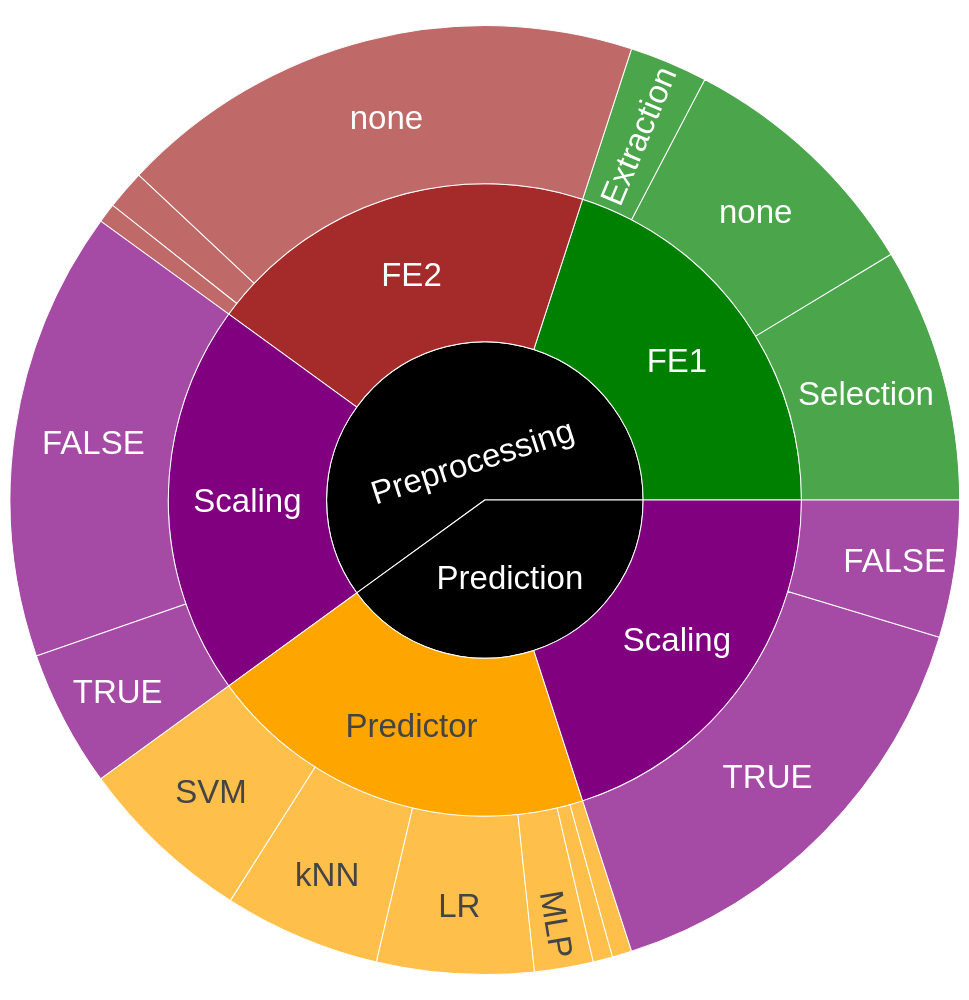
\includegraphics[width=5.5cm]{img/sunburst/cv.png}
    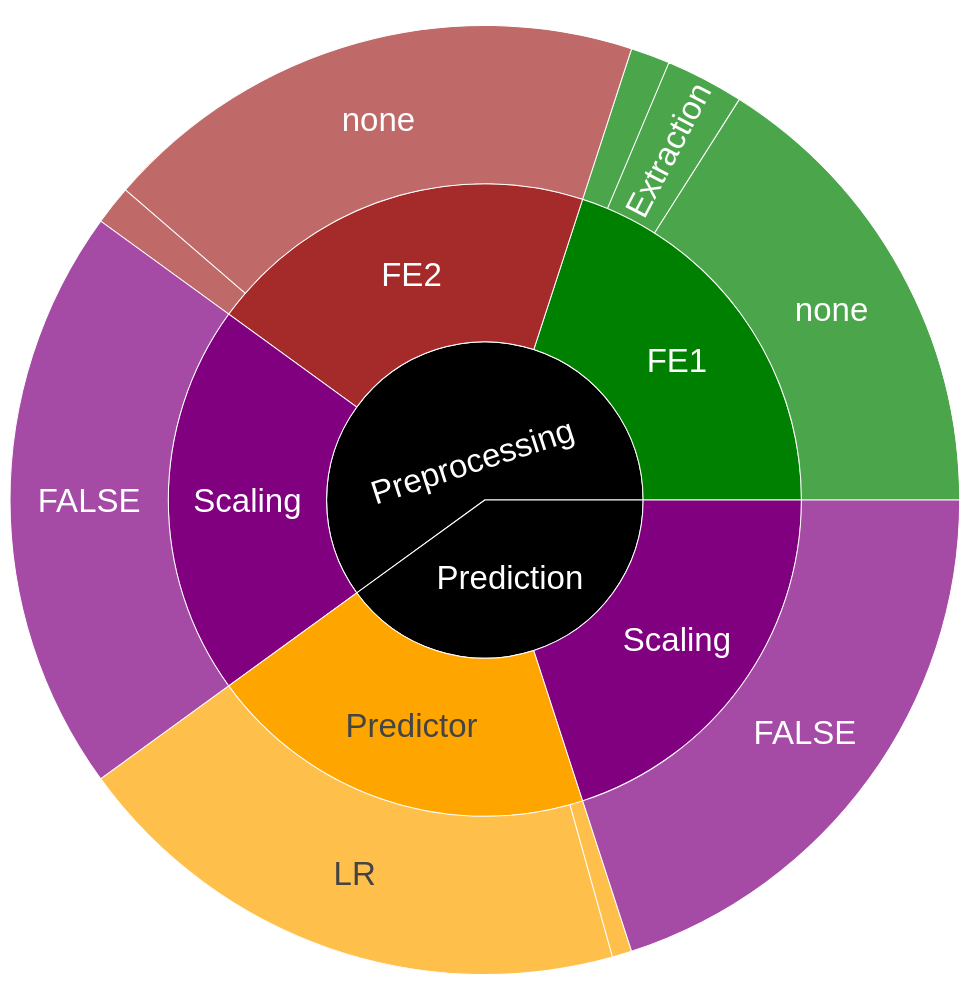
\includegraphics[width=5.5cm]{img/sunburst/nlp.png}
    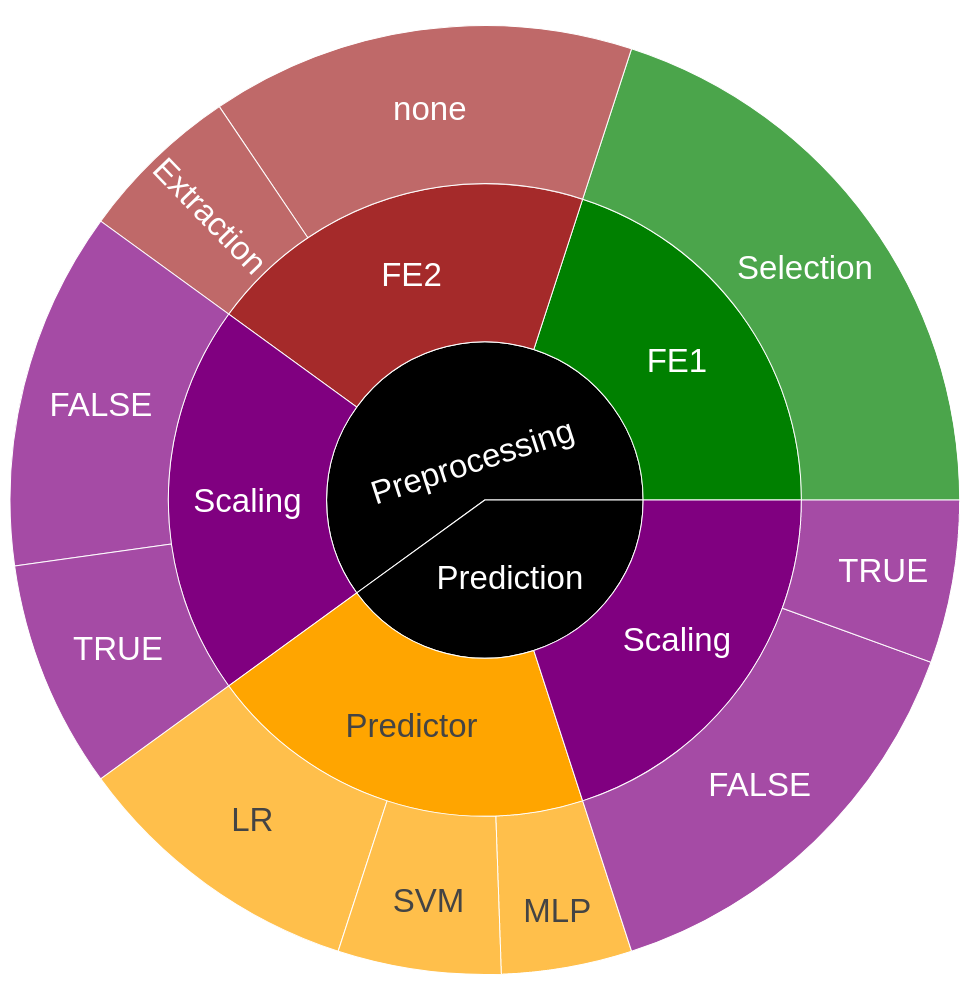
\includegraphics[width=5.5cm]{img/sunburst/ts.png}
    \caption{Pipeline composition for the different domains considered. From left to right: CV, NLP, and TS.}
    \label{fig:domain_composition}
    
    % [CV] prediction: LR (cifar10), SVM (fmnist), kNN (svhn)
    % [CV] preprocessing: increasingly used, in this order
    % 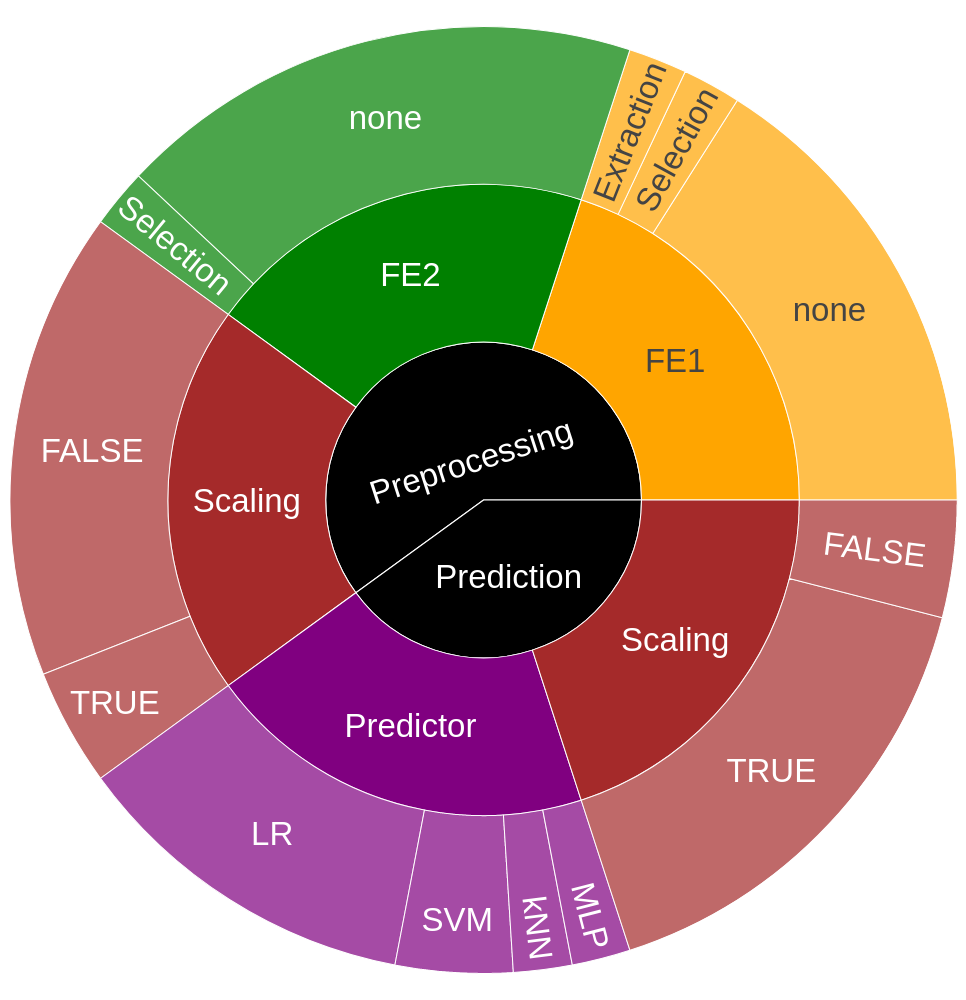
\includegraphics[width=5.5cm]{img/sunburst/cifar10.png}
    % 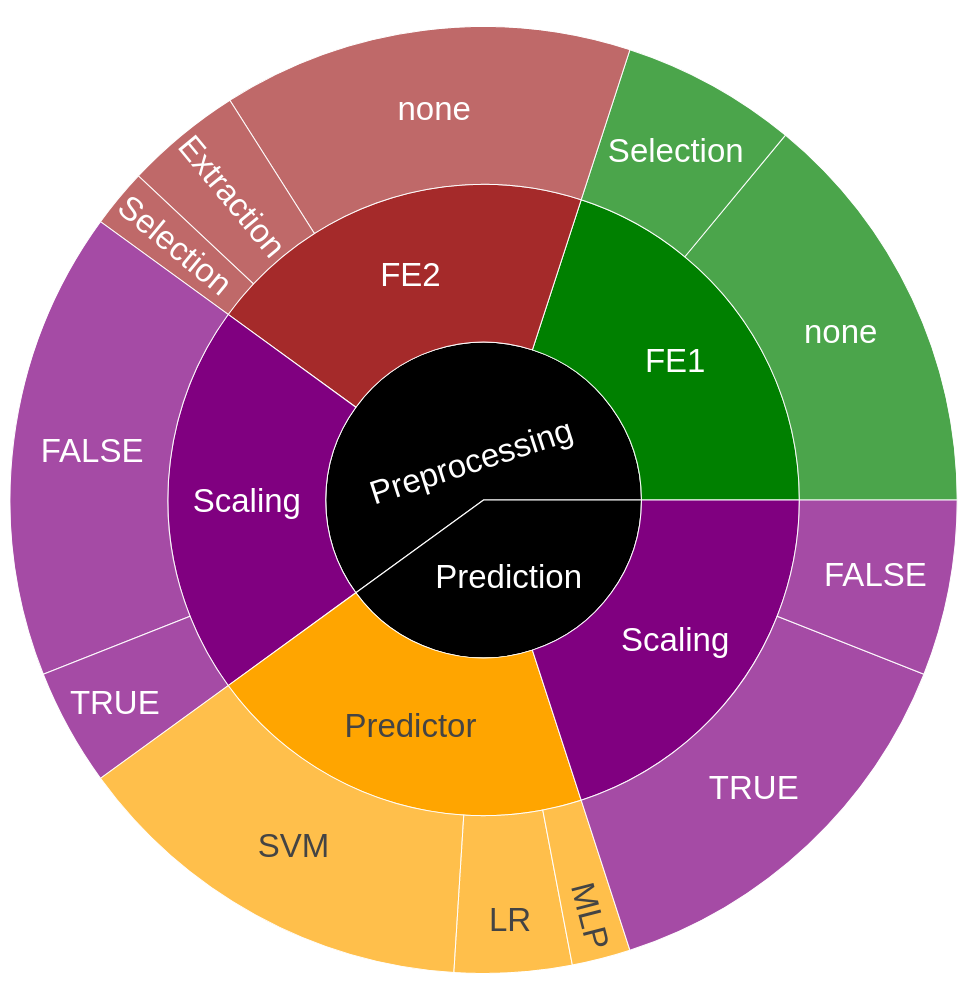
\includegraphics[width=5.5cm]{img/sunburst/fmnist.png}
    % 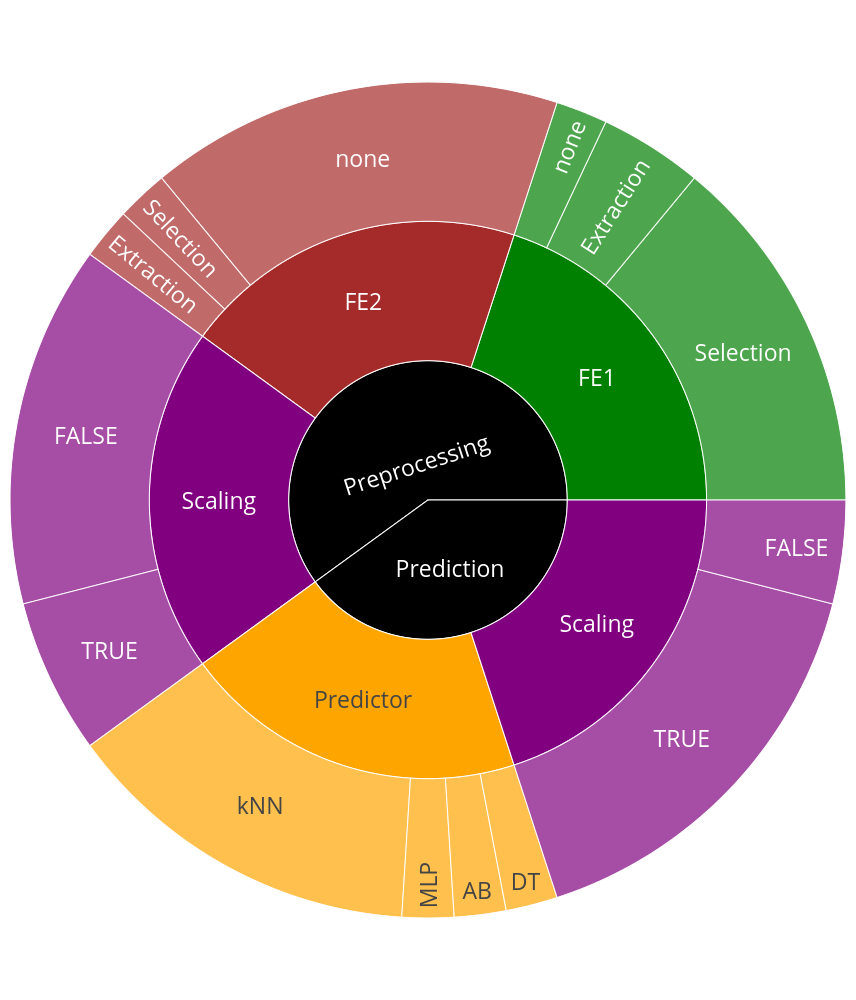
\includegraphics[width=5.5cm]{img/sunburst/svhn.png}
    
    % [TS] prediction: LR + SVM + MLP (natal), LR + SVM (boston)
    % 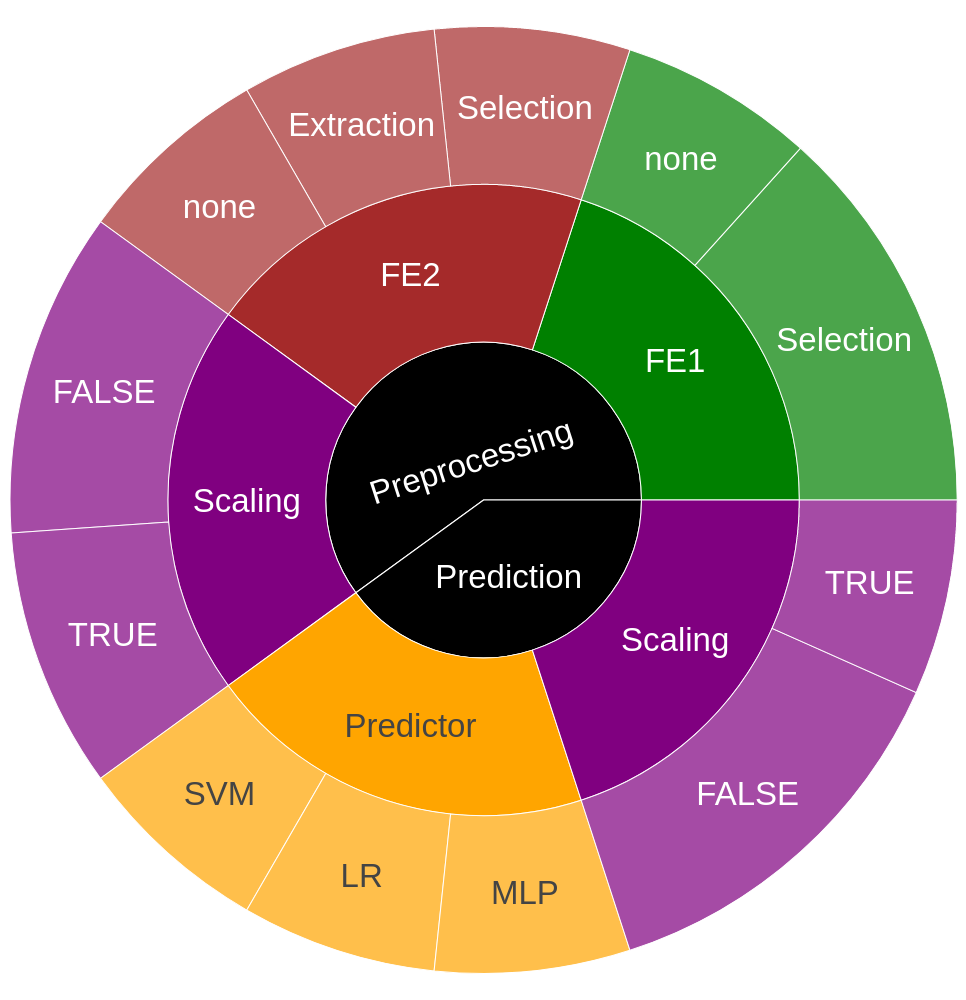
\includegraphics[width=5.5cm]{img/sunburst/natal.png}
    % 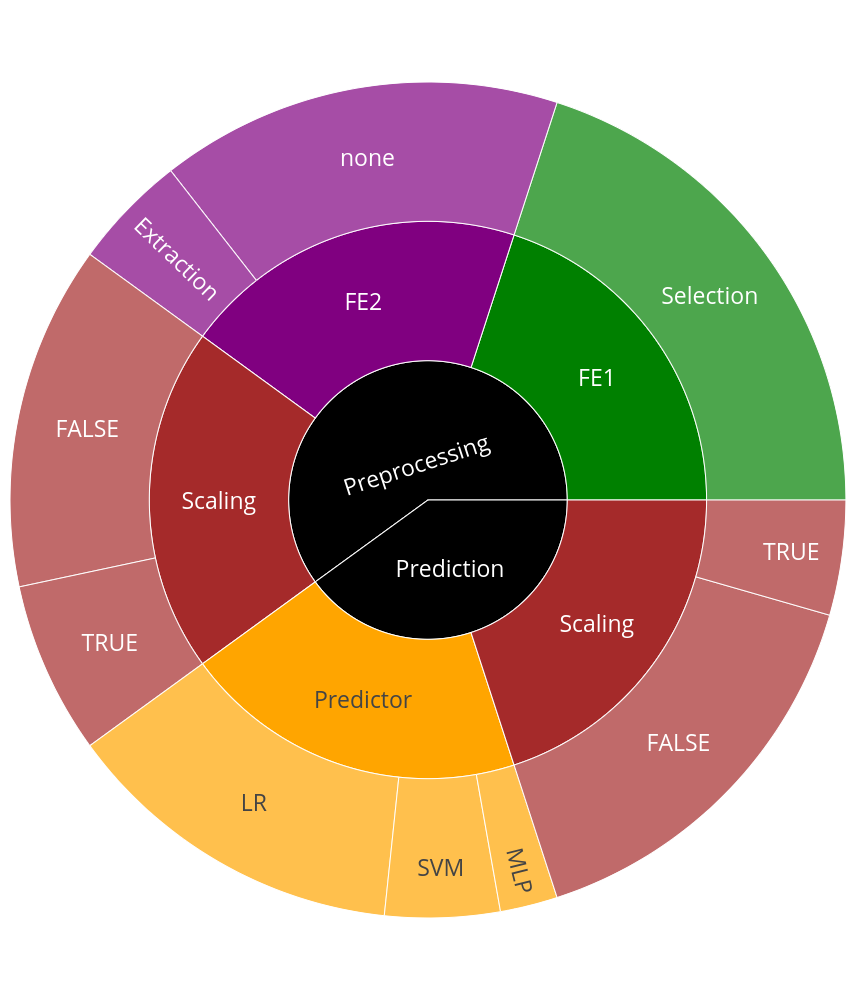
\includegraphics[width=5.5cm]{img/sunburst/boston.png}
    
    % [NLP] preprocessing: extraction -> selection (reuters)
    % 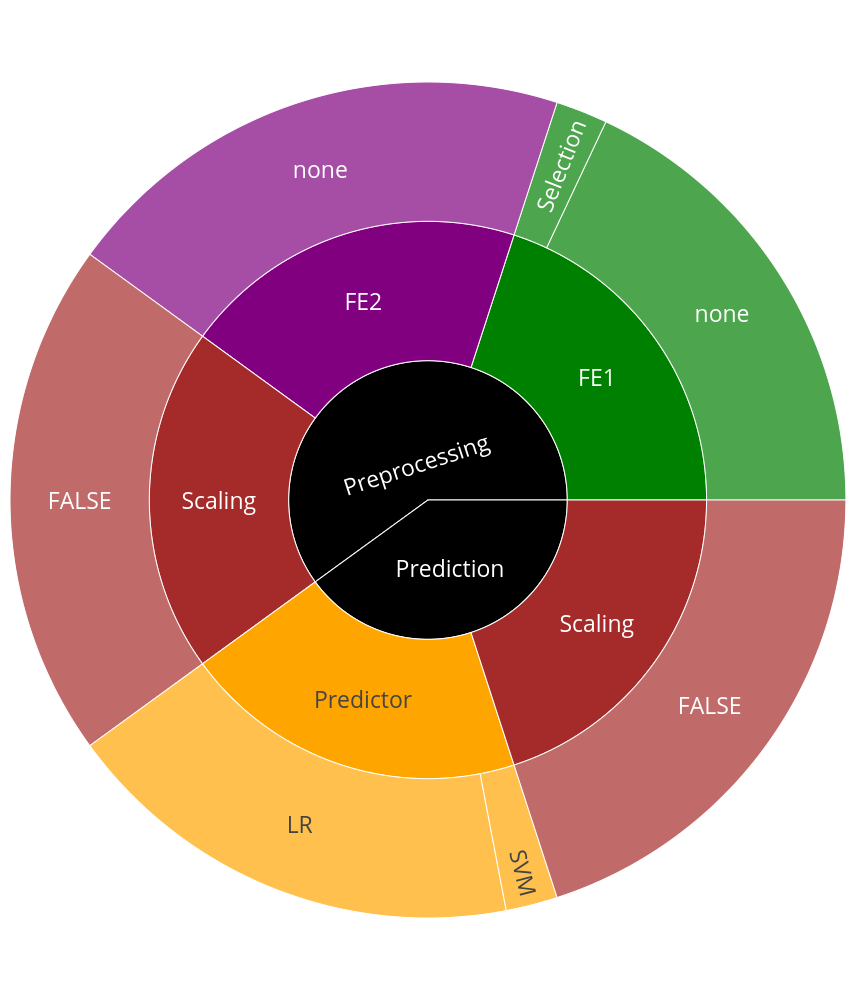
\includegraphics[width=5.5cm]{img/sunburst/lmrd.png}
    % 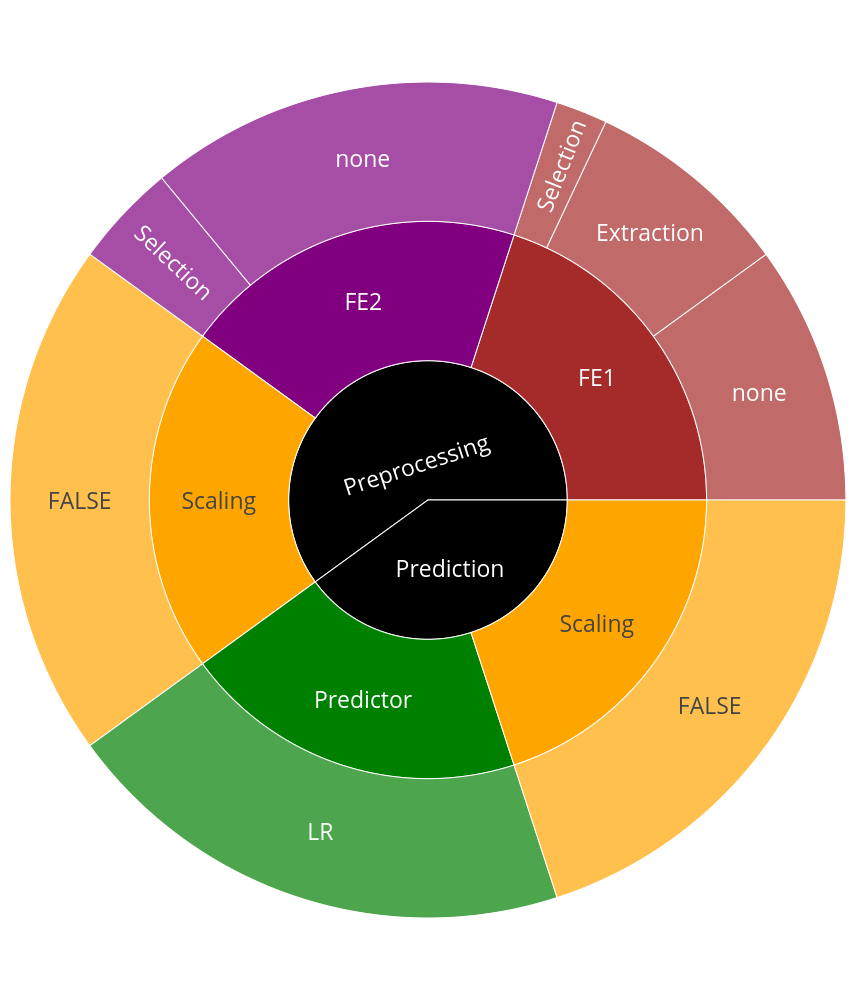
\includegraphics[width=5.5cm]{img/sunburst/reuters.png}
    % 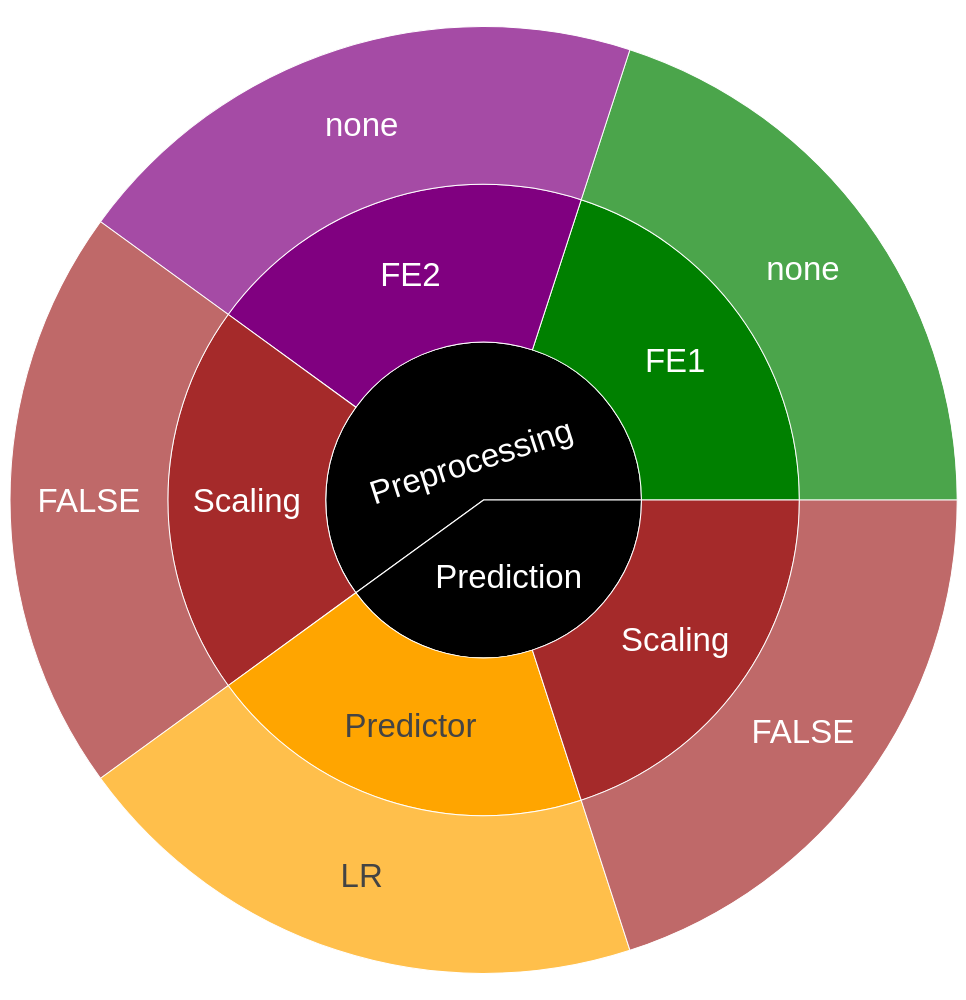
\includegraphics[width=5.5cm]{img/sunburst/agnews.png}
\end{figure*}

The compositions discussed above constitute strong evidence for the benefits of AutoML tools over manual selection and configuration. In addition, the simplicity of our template greatly improves the understanding of the pipelines selected. Finally, some of these observations might suggest the maximum runtime we fixed for each experiment for feasibility affects the composition of the pipelines. This possibility is further explored in Section~\ref{sec:alt-setups}. Nonetheless, the comparison of final scores for each dataset given in Table~\ref{tb:results} confirms that these pipelines are indeed high-performing w.r.t.~the provided configuration space and setup. Accuracy scores given for classification problems, as well as $R^2$ scores given for regression problems, are to be maximized. The best value per dataset is given in boldface. 

\begin{table*}[]
\centering
\caption{Accuracy~(\%) and $R^2$ scores (mean $\pm$ stand. deviation) for each dataset. The best algorithm per dataset is highlighted in boldface.}
\label{tb:results}
\scalebox{0.8}{\begin{tabular}{r|c|c|*{7}{c}|cc}
\hline  
\emph{Task} & \emph{Domain} & \emph{Dataset} & KNN & DT & RF & AB & MLP & SVM & LR & \isklearn & \textsc{AutoSklearn}\\ \hline
\multirow{6}{*}{\emph{Classification}} & \multirow{3}{*}{\emph{CV}} 
% & \emph{MNIST} & 96.88 & 87.76 & 94.16 & 72.99 & 95.82 & 11.35 & --- & \textbf{98.60} & 97.67\\ 
% \cline{3-12}
 & \emph{CIFAR-10} & 32.98 & 26.78$\pm0.27$ & 34.61$\pm0.35$ & 31.08 & 34.21$\pm0.37$ & 20.44 & 30.24 & 43.96$\pm6.95$ & \textbf{50.55}$\pm9.44$ \\ 
\cline{3-12}
%  & & \emph{CIFAR-100} & 15.04 & 08.48 & 13.39 & 07.03 & 01.00 & 04.50 & --- & \textbf{20.50} & \\ \cline{3-12}
 & & \emph{FMNIST} & 85.54 & 79.05$\pm0.17$ & 85.44$\pm0.14$ & 54.25 & 84.87$\pm0.52$ & 10.02 & 80.12 & \textbf{88.12}$\pm2.24$ & 79.88$\pm5.48$ \\ \cline{3-12}
 & & \emph{SVHN} & 46.83 & 42.17$\pm0.22$ & 56.51$\pm0.38$ & 22.78 & 19.58$\pm0.00$ & 0.00 & 23.94 & \textbf{58.02}$\pm15.52$ & 53.25$\pm10.41$ \\ \cline{2-12}
 & \multirow{3}{*}{\emph{NLP}} & \emph{LMRD} & 67.20 & 70.23$\pm0.15$ & 73.00$\pm0.64$ & 80.31 & 86.29$\pm0.09$ & 63.29 & 88.31 & \textbf{88.32}$\pm0.19$ & 88.01$\pm0.19$\\ \cline{3-12}
 &  & \emph{Reuters} & 77.74 & 70.41$\pm0.38$ & 69.32$\pm0.77$ & 47.55$\pm0.14$ & 80.59$\pm0.19$ & 36.20 & 79.07 & 81.57$\pm0.35$ & \textbf{82.57}$\pm1.01$ \\ 
 \cline{3-12}
 &  & \emph{AGNews} & 90.20 & 75.97$\pm0.22$ & 84.06$\pm0.41$ & 68.24 & 91.07$\pm0.19$ & 72.30 & 91.39 & \textbf{91.74}$\pm0.07$ & 91.57$\pm0.9$ \\ 
 \hline
\multirow{2}{*}{\emph{Regression}} & \multirow{2}{*}{\emph{TS}} & \emph{Natal} & 0.94 & 0.9134$\pm0.0022$ & 0.9538$\pm0.0047$ & 0.9185$\pm0.0089$ & 0.9547$\pm0.0016$ & 0.9389 & \textbf{0.9575} & 0.9538$\pm0.0022$ & 0.9549$\pm0.0087$\\
\cline{3-12}
 & & \emph{Boston} & 0.9576 & 0.9428$\pm0.0009$ & 0.9634$\pm0.0004$ & 0.9440$\pm0.0023$ & 0.9728$\pm0.0021$ & 0.8454 & 0.9743 & \textbf{0.9751}$\pm0.0001$ & 0.9707$\pm0.0006$\\
% \cline{2-12}
% & --- & \emph{NYC} & 0.6095 & 0.4477 & 0.6797 & 0.3821 & 0.5811 & 0.5495 & 0.4270 &  & 0.6991\\ 
\hline
\end{tabular}}
\end{table*}
As expected, pipelines devised by \isklearn and ensembles devised by \autosklearn present better performance than default models. The only exception is the Natal dataset, for which LR outperforms both AutoML tools. Comparing \isklearn and \autosklearn, it is remarkable that pipelines from the former are competitive with the ensembles from the latter. Indeed, the only datasets for which we see a non-negligible gap between the performance of the models devised by the two AutoML approaches are the three CV ones. For CIFAR-10, ensembles present higher mean, though at the cost of higher variance as well. For FMNIST and SVHN, it is the pipelines that achieve higher mean, though again at the cost of higher variance for the latter. Altogether, these results evidence the difficulty posed by computer vision problems when deep learning is not adopted. One likely explanation is the computational cost incurred by sample dimensionality, which becomes more critical in runtime-constrained scenarios. 
%Regarding Reuters, experiments reported on the supplementary material demonstrate that \irace initially converges to one or two predictors and then fine-tunes hyperparameters. In this case, \irace selected a well-performing predictor, based on the performance of the default models, but configuring MLPs is computationally costly, and likely would require more resources.

From a practical point of view, most of the pipelines engineered in this section could be deployed into a real-world production setup, due to their simplicity and performance. The only exceptions are CIFAR-10 and SVHN, for which both the pipelines from \isklearn and ensembles from \autosklearn still require improvements to produce estimators with a reasonable level of effectiveness.
%, which we investigate in the next section. 
In the next section, we investigate the effects of our proposed configuration space and setup in the performance of \isklearn.%, with a particular focus on CV. %Some of those experiments are also performed for NLP and TS, as we will discuss.

% !TEX root = ../main.tex

\section{Ablating \isklearn}
\label{sec:further}

Results from the first part of our investigation validated our \irace AutoML proposal as a competitive approach in terms of efficacy. We next ablate \isklearn to understand how the proposed configuration space and setup affect its performance. We start with a configuration space analysis,  where we assess the benefits of having a minimalist template. Later, we appraise different configuration setups, exploring the idea of the generalized mid-level sampling and providing guidelines for the application of \isklearn to other problems.

% Yet, CIFAR-10 results indicate that further investigation is required on more challenging domains, such as computer vision. In this section, we assess~(i)~alternative configuration setups and~(ii)~the feasibility of transfer learning. The datasets adopted in this section were chosen for their popularity in the small image classification literature. Specifically, we replace MNIST with Fashion MNIST~(FMNIST), given the small margin for improvement on the former. In addition, we also consider CIFAR-100, a dataset similar to CIFAR-10, and SVHN, a house number recognition problem. Further information on these datasets is given in the supplementary material, particularly the details on manual data preparation, sampling, and resource limits for \autosklearn.

%\input{sections/transfer-learning}
\subsection{Comparing configuration spaces}

To assess the benefits of having a simpler template in terms of efficacy of the pipelines produced, we use SMAC~\cite{smac} to configure pipelines from our template. Since SMAC is the configurator powering \autosklearn, the comparison given in Figure~\ref{fig:smac} helps us isolate the effects of configurator and templated adopted. We focus this investigation on CV datasets as they were the most challenging for both AutoML approaches.

\begin{figure}
    \centering
    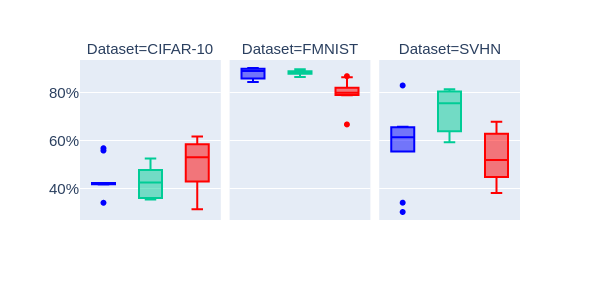
\includegraphics[width=\linewidth, clip=true, trim=45px 80px 80px 40px]{img/smac.png}
    \caption{Accuracy comparison between pipelines configured by \tinyirace~(blue) and SMAC~(green) from \tinyisklearn and ensembles configured by SMAC from \autosklearn~(red).}
    \label{fig:smac}
\end{figure}

Boxplots for the different datasets indicate that the performance of pipelines configured from \isklearn by SMAC are more similar in performance to pipelines configured from \isklearn by \irace than to the ensembles configured from \autosklearn by SMAC itself. 
% Interestingly, the distributions of the accuracy scores for the pipelines configured by SMAC and \irace are very different, with quartiles for \irace being located closer to their median than for SMAC, but presenting strong outliers. 
More repetitions of these experiments would be required to understand if the differences in distributions between \irace and SMAC results are consistent, or if the outliers observed are fluctuations in the experiments. Nonetheless, the comparison between pipelines and ensembles confirms that our proposed minimalist template is a contribution not only in terms of simplicity and interpretability, but also as to efficacy. Furthermore, it evidences the generality of the configuration space and setup proposed, as they can be coupled with any configurator that supports numerical, categorical, and conditional parameters, such as SMAC.

% !TEX root = ../main.tex

\subsection{Alternative Configuration Setups}
\label{sec:alt-setups}

Results discussed in Section~\ref{sec:results} indicated the efficacy of the configuration setup adopted, but some relevant questions need to be further investigated. We start with the analysis of the TS datasets. Our goal is to understand the impact of the different sampling generalization approaches we propose, in particular the bottom-level sampling cross-validation approach that should suit TS problems better than the traditional holdout.
Figure~\ref{fig:ts-setups} gives boxplots of experiments where we compare the original setup adopted in Section~\ref{sec:results}~(dubbed \textbf{regular}) and a setup where we increase the number of meta-folds to $p=3$ and total cutoff time to 15min~(dubbed~\textbf{TM}, for \textit{triple meta-fold}). For brevity, a discussion on the balance between the number of meta-folds and total cutoff time is provided as supplementary material.
% ADD TO SUPP!
%This change in setup aims to provide more samples to the bottom-level sampling, and thus reduce the chance of overfitting. However, having three times more samples incurs in a cutoff time issue for the evaluation of the meta-folds. On one hand, reusing the 10min total cutoff time from \textit{regular} would mean the cutoff time per meta-fold would be reduced to roughly 3min. On the other hand, preserving the cutoff time per metafold at 10min would increase the total cutoff time to 30min. In this initial experiments, we adopt a middle ground solution and set total cutoff time to 15min, which translates into 5min per-meta-fold cutoff time.
%
%where we reduce the number of setups considered, but include ensembles produced from \autosklearn as baseline. 
The \textbf{regular} setup is given in blue, whereas the \textbf{TM} setup is given in red. Since it is not possible to configure the number of meta-folds used for bottom-level sampling in \autosklearn, results provided for ensembles under \textbf{TM} reflect only the increase in total cutoff time. 

\begin{figure}
    \centering
    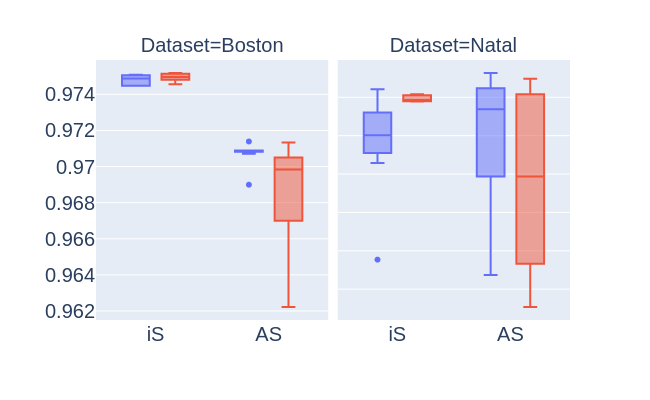
\includegraphics[width=0.8\linewidth, clip=true, trim=45px 50px 80px 30px]{img/ts-setups.png}
    \caption{R$^2$ comparison of \tinyisklearn and \autosklearn on TS datasets using different configuration setups. Blue: \textbf{regular}; red: \textbf{TM}.}
    \label{fig:ts-setups}
\end{figure}

As previously discussed, the best-performing AutoML tool for the \textbf{regular} setup varies as a function of the TS dataset considered. However, under the \textbf{TM} setup the pipelines from \isklearn outperform the ensembles from \autosklearn for all datasets.
%(even if \autosklearn has more cutoff timavailable for the evaluation). 
These results are explained by two factors. First, the performance of \isklearn pipelines is improved by the inclusion of more meta-folds, even if proportionally the cutoff time for the evaluation of each meta-fold is halved. Second, the performance of \autosklearn ensembles is reduced by the increase in cutoff time. One likely explanation is that the larger training time enables SMAC to select more complex ensembles, which tend to overfit in a time series setup using holdout.

To further investigate the impact of cutoff time and number of meta-folds, we extend our experimental design. Besides those factors, we also investigate the impact of increasing the total number of experiments \irace is allowed to perform. 
%  to comprise three experimental factors: 
%setups where we~(i)~reduce the chances that candidate evaluation is not completed within the cutoff time; (ii)~allow \irace to evaluate a larger number of candidate configurations, and/or; (iii)~assess our mid-level sampling generalization proposal, intended to provide the bottom-level sampling more data and thus reduce the chance for overfitting. 
% Our rationale is that CIFAR-10 was the most computationally demanding dataset in the previous section, and hence increasing the resources provided to \isklearn should lead to better-performing pipelines. 
%
%To accomplish these goals, we consider three experimental factors, namely 
%increased (i)~cutoff time, (ii)~configuration budget, and (iii)~number of meta-folds~($p$). 
Table~\ref{tab:exp-configs} depicts the setups we produce from these factors, where \textbf{regular} serves as baseline. With \textbf{20m}, \textbf{5k} and \textbf{TM 30m} we independently investigate increased (i)~cutoff time, (ii)~configuration budget, and (iii) number of meta-folds, respectively. In addition, since a total cutoff time of 30m may be impractical depending on the computational setup available, we investigate with \textbf{TM} and \textbf{TM 5k} whether halving the total cutoff time would be an option. For instance, the TS analysis above adopted \textbf{TM}, where halving the total cutoff time was compensated by the increased number of meta-folds.

% Setups dubbed \textbf{TM}~(short for \textit{triple meta-fold}) use $p=3$, i.e., the mid-level sampling procedure uses three meta-folds. Additionally, two setups allow increased configuration budget (\textbf{5k} and \textbf{TM 5k}), with 5000 experiments allowed instead of the previous 2000. Lastly, setups that consider increased cutoff time~(\textbf{20m} and \textbf{TM 30m}) allow for a doubled cutoff time w.r.t. their corresponding reference setups~(\textbf{regular} and \textbf{TM}, respectively).
% Complementarily, accuracy results for each setup~(columns) and dataset~(rows) are given in Table~\ref{tb:further-accuracy}. The best value obtained per benchmark among \isklearn pipelines is highlighted in boldface, and accuracies of ensembles from \autosklearn are also highlighted when they outperform all pipelines from \isklearn for the given benchmark. 

\begin{table}[!t]
\centering
\caption{Summary of the six configuration setups considered in this section. Regular~(\textbf{reg}.) stands for the configuration setup assessed in the previous section, used here as baseline.}
\label{tab:exp-configs}
\scalebox{0.85}{\begin{tabular}{r*{7}{c}}
\hline
\textbf{setup} & \textbf{reg.} & \textbf{20m} & \textbf{5k} & \textbf{TM 30m} & \textbf{TM} & \textbf{TM 5k}\\ \hline
\textbf{$p$} & 1 & 1 & 1 & 3 & 3 & 3 \\ \hline
\textbf{budget} & 2000 & 2000 & 5000 & 2000 & 2000 & 5000 \\ \hline
\textbf{cutoff} & 10m & 20m & 10m & 30m & 15m & 15m \\ \hline
\end{tabular}}
\end{table}

% When cutoff time was OK (Reuters), no experimental factor helped consistently, though more samples worsened performance slightly.
% CIFAR-10 results are outliers, likely because of the large gap to the state-of-the-art
% Increasing the number of experiments helps
% Increasing the number of samples helps, except for FMNIST where it is irrelevant
% Reducing cutoff time in general worsens performance, but the increased number of experiments helps, sometimes greatly FMNIST

% CT: if cutoff time was enough, doubling shouldn't affect greatly
% - Cutoff time was OK: Reuters
% - Cutoff time was not enough: CIFAR-10, FMNIST, SVHN, LMRD, AGNews
% 5k: if number of experiments was enough, increasing shouldn't affect greatly
% - Cutoff time was not enough, and more experiments didn't help: CIFAR-10
% - Cutoff time was not enough, but more experiments helped: FMNIST, SVHN, LMRD, AGNews
% TM: if number of samples was enough, tripling shouldn't affect greatly 
% - Cutoff time was not enough, and more samples didn't help: CIFAR-10, FMNIST
% - Cutoff time was not enough, but more samples helped: SVHN, AGNews

Boxplots given in Figure~\ref{fig:setups} depict accuracy scores for CV~(left column) and NLP~(right column) datasets, on which we focus due to the larger improvement margins observed in Section~\ref{sec:results}. However, margins as large as CIFAR-10 make results for this dataset outliers, and hence the following discussion focuses on the remaining ones. For a given plot, setups are ordered as in Table~\ref{tab:exp-configs}. We first remark that the differences in performance among setups is much more significant for CV datasets than for NLP ones. Apart from that, the most important factor observed was cutoff time, as only for Reuters we do not observe improvements under setup \textbf{20m}. For this dataset, none of the remaining factors consistently helped, though adopting more samples worsened performance slightly. For the remaining datasets, increasing either the number of experiments~(\textbf{5k}) or the number of meta-folds~(\textbf{TM}) improved performance. The only exception was FMNIST, for which increasing the number of meta-folds changed performance to a negligible rate. Finally, reducing the cutoff time did not compensate for the increased number of meta-folds~(\textbf{TM}), though the possibility of more experiments~(\textbf{TM 5k}) alleviated the loss in performance. Once again, FMNIST was an exception, since results under \textbf{TM 5k} were even better than for \textbf{TM 30m}.
% CIFAR-10 results are outliers, likely because of the large gap to the state-of-the-art
% Increasing the number of experiments helps
% Increasing the number of samples helps, except for FMNIST where it is irrelevant
% Reducing cutoff time in general worsens performance, but the increased number of experiments helps, sometimes greatly FMNIST

% For a given plot, setups are ordered as in Table~\ref{tab:exp-configs}. Results present interactions between application domain, dataset, and the experimental factors used to produce the setups we assess. Concerning application domain, the CV datasets seem to be more sensitive to configuration setup changes than the NLP ones. Furthermore, patterns are not consistent, even for datasets from the same domain. Still, we can observe overall that increasing configuration budget or cutoff time in single meta-fold setups mostly improves results. Similarly, the triple meta-fold approach can be useful, but often only if combined with increased configuration budget or cutoff time. This shows that while an increase in configuration budget or cutoff time is not necessary for experimental purposes, it might be desirable for certain applications.

\begin{figure}
    \centering
    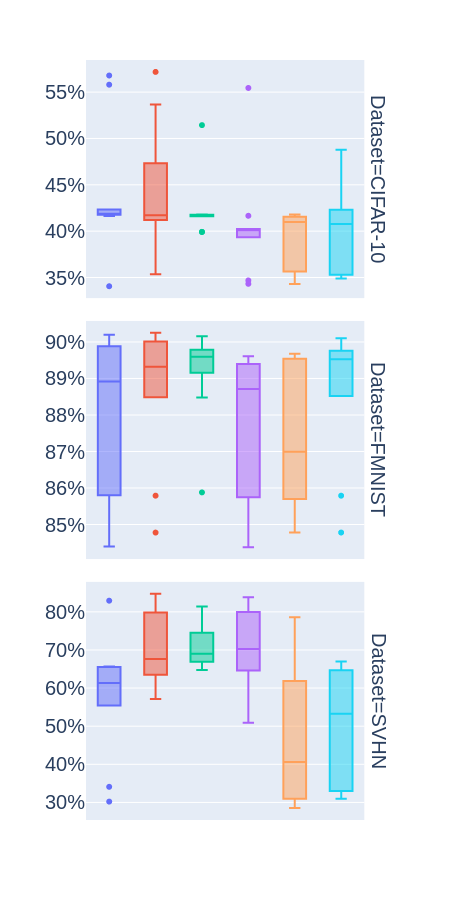
\includegraphics[width=0.49\linewidth, clip=true, trim=45px 70px 45px 60px]{img/cv-setups.png}
    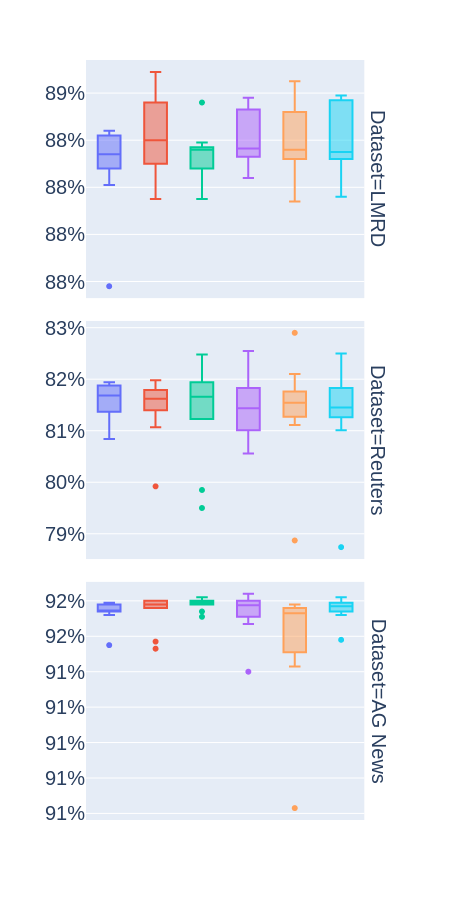
\includegraphics[width=0.49\linewidth, clip=true, trim=45px 70px 45px 60px]{img/nlp-setups.png}
    \caption{Accuracy comparison on CV~(left column) and NLP~(right column) datasets under alternative configuration setups. Within each plot, setups are ordered as in Table~\ref{tab:exp-configs}.}
    \label{fig:setups}
\end{figure}

% In general, 
% single meta-fold (SM) setups~(setups where the number of meta-folds $p=1$) are preferable to our previous approach~($p=3$). Do note that, while trends point to more favorable results with the single meta-fold approach, results about other factors are inconclusive. Specifically, increasing the number of experiments and/or the cutoff time does not necessarily lead to better results.
% Nonetheless, it is remarkable that changes to the configuration setup lead to a 42.32\% accuracy improvement on CIFAR-10 and to  21.73\% on SVHN. In fact, the improvement on CIFAR-10 leads to an accuracy higher than that of \autosklearn, which is also true for CIFAR-100. The most extreme situations concern FMNIST and SVHN, where performances are considerably different between pipelines from \isklearn and ensembles from \autosklearn. Further investigation on these datasets would be required to understand these significant gaps, but exceed the scope of this work. 

% \medskip
% Altogether, the experiments in this section have helped understand the impact of the different components of \isklearn. 
% Altogether, the experiments in this section indicate that the first configuration setup factor a practitioner should try to adjust is the cutoff time for a single experiment. If that is not feasible due to computational setup limitations, increasing the number of meta-folds can be an effective alternative, confirming the contribution of our generalized sampling.

% \begin{table}[]
% \centering
% \caption{Accuracy for each dataset/configuration setup pair. Ensembles produced by \autosklearn~(AS) are taken as baseline.}
% \label{tb:further-accuracy}
% \scalebox{0.78}{\begin{tabular}{r|*{6}{c}|cc}
% \hline
%  & \textbf{reg.} & \textbf{5k} & \textbf{30m} & \textbf{SM} & \textbf{SM 5k} & \textbf{SM 20m} & \textsc{AS} \\ \hline
% \textbf{C10} & 35.73 & 43.61 & 40.15 & \textbf{50.85} & 43.24 & 32.13 & 48.30 \\ \hline
% \textbf{C100} & 20.50 & 20.54 & 17.88 & 19.58 & 16.80 & \textbf{21.14} & 18.89 \\ \hline
% \textbf{FM} & 88.63 & 87.64 & 85.23 & 88.26 & 88.99 & \textbf{89.18} & \textbf{97.27} \\ \hline
% \textbf{SVHN} & 65.89 & 72.82 & 66.7 & 65.33 & \textbf{80.21} & 55.10 & 41.14\\ \hline
% \end{tabular}}
% \vspace{-12pt}
% \end{table}


% We next proceed to the pipeline composition assessment given in Table~\ref{tb:further-predictor}, where again rows depict benchmarks and columns the different experimental setups considered. Each cell lists the feature engineering~(\textsf{\footnotesize FE}) components (when used and, if so, in which order), and  predictors~(\textsf{\footnotesize Pred}) selected by \irace.
% Patterns in this table are much more clear. Concerning pre-processing, over two thirds of the cells include some FE component. Surprisingly, even if extraction is expected to be effective for computer vision problems, only half of the pipelines that include FE comprise extraction. More importantly, none of the pipelines that are best-performing for each benchmark use extraction. Among the best-performing pipelines, three out of four adopt feature selection, but differ as to how. 

% \begin{table}[!t]
% \centering
% \caption{Feature engineering (FE) and prediction (Pred) components selected for each dataset/configuration setup pair.}
% \label{tb:further-predictor}
% \scalebox{0.8}{\begin{tabular}{r*{8}{c}}
% \hline
% & & \textbf{reg.} & \textbf{5k} & \textbf{30m} & \textbf{SM} & \textbf{SM 5k} & \textbf{SM 20m}\\ \hline
% \multirow{2}{*}{\textbf{C10}} & \textsf{FE} & - & E & S\&E & \textbf{S} & E\&S & - \\
% & \textsf{Pred} & kNN & kNN & kNN & \textbf{SVM} & kNN & AB \\ \hline
% \multirow{2}{*}{\textbf{C100}} & \textsf{FE} & E & E\&S & - & - & S & \textbf{S} \\
% & \textsf{Pred} & kNN & kNN & DT & MLP & kNN & \textbf{MLP} \\ \hline
% \multirow{2}{*}{\textbf{FM}} & \textsf{FE} & S & - & S & E\&S & - & \textbf{-} \\
% & \textsf{Pred} & MLP & MLP & SVM & MLP & MLP & \textbf{MLP} \\ \hline
% \multirow{2}{*}{\textbf{SVHN}} & \textsf{FE} & S & S\&E & S & S & \textbf{S} & S \\
% & \textsf{Pred} & kNN & kNN & kNN & kNN & \textbf{SVM} & kNN \\ \hline
% \end{tabular}}
% \end{table}

% Regarding predictors, $k$-nearest neighbors~(kNN) is selected half of the times, although none of the best-performing pipelines are based on kNN. Yet, while this is a relatively simple prediction algorithm, most of the kNN-based pipelines use some of form of FE. Combined, these components lead to competitive performance on CIFAR-100 and Fashion MNIST w.r.t. the other pipelines. Out of the prediction algorithms that were in fact chosen in the best-performing pipelines, SVM and MLP are equally occurring. Altogether, these designs indicate that \isklearn balances the computational cost of its different components.
%The success of the latter might be correlated with the overall success of other more complex neural networks in computer vision problems. As for the former, SVMs had already been select on two out of three datasets of different domains, in our previous experiments.


%\cleardoublepage
%!TEX root = ../main.tex

\section{Conclusion}
\label{sec:conclusion}

Automated machine learning~(AutoML) is a growing research field both as to the number of tools available and to the results they help achieve. One of its main goals is to bridge non-experts and the specialized knowledge underlying successful ML applications. Another, equally important, is to reduce the computational/environmental cost currently incurred by the ML industry. Overall, AutoML approaches stem from research fields as diverse as algorithm configuration, neuroevolution, and neural architecture search. Yet, the proposal and assessment of these approaches need to be aware of their cost.

In this work, we have conducted an experimental investigation with these two goals in mind, attempting to maximize the number of insights observed from our work while keeping the number of experiments constrained. In this context, we have empirically demonstrated how \irace can be used to configure pipelines that outperform the predictors that comprise it, considering several relevant application domains, such as computer vision, natural language processing, and time series analysis. Even if the goal of the paper is not to benchmark AutoML approaches, it is remarkable that the pipelines engineered from \isklearn displayed competitive performance w.r.t. more elaborate ensembles produced by the well-known \autosklearn. 
Furthermore, our minimalist configuration space proved helpful both as to effectiveness and to interpretability of pipeline composition. Finally, we assessed different configuration setups and discussed the different options a practitioner can employ to further improve efficacy. 
%Interestingly, the insights we observe confirm what had been reported in the literature about transfer learning between neural networks, even if we consider a larger sample of predictors.

Our work aimed to be comprehensive, and so many of the insights we observed deserve future investigation. The first is pushing further the idea of environment-aware AutoML research. Indirectly, this effort has been driven by the desire to bring machine learning models to mobile hardware. One emblematic example is multi-objective neuroevolution, which evolves models to simultaneously optimize these two goals. Concerning algorithm configuration AutoML approaches, \irace is an important asset in this task, as it 
has been effectively employed for multi-objective configuration~\cite{BezerraPhD,BezLopStu2020}. 

A second path for future work is to investigate machine learning-specific setups for irace. Here, we have observed that variations to the setup adopted affect the performance of the pipelines produced, specially for computer vision problems. A likely promising direction is to mimic deep learning training, where models are repeatedly exposed to the same dataset. In the context of \isklearn, this would translate into resuming training when a candidate pipeline needs to be evaluated on the same meta-fold again. The main challenge with this alternative is to balance effectiveness with the costs it incurs.

% A third path of investigation concerns transfer learning and its impact may not be limited to \isklearn. Specifically, effective transfer learning between neural networks has generally relied on (i)~large-scale source datasets and (ii)~fine-tuning for co-adapting neurons. In this work, neither of these assets have yet been adopted. Concerning the former, it would be trivial to produce variants of existing large image datasets such as ImageNet or Faces in the Wild for small image classification. Regarding fine-tuning, it remains to be investigated how pipelines produced from \isklearn could be used as a source for backpropagation to the reused network.

Finally, while our investigation has focused on AutoML effectiveness, it is also imperative to pursue robustness. More precisely, in this investigation we have sought to include problem datasets from diverse applications domains. Yet, every dataset we have considered was initially subject to some extent of manual data preparation. Other AutoML tools, such as \autosklearn, aim to automate even this part of the process. Considering the importance of data preparation, its relevance to predicting performance, and the reduced computational cost of this stage, making available a data preparation module to be coupled with \isklearn is an important path of future work.

%Automated algorithm engineering approaches seek to bridge the gap between non-experts and the specialized knowledge underlying successful soft computing  applications. The case of automated machine learning~(AutoML) is a rather emblematic successful example, with industry and academia working together to popularize the field. Although many tools are already available for the general public, the efficacy of those tools must be continuously improved by the research community. For this purpose, the algorithm configuration community has devised a number of efficient tools over the past years that have been seldom (if at all) explored in the context of (automated) machine learning. 
%
%\irace is one such tool, having become one of the most used and efficient algorithm configurators currently available. Indeed, it is rather unfortunate that no AutoML tool powered by \irace had been proposed so far, particularly due to its setup flexibility and ability to deal with different types of parameters. In this work, we have conducted a first effort in this direction, covering all aspects required to use \irace in the context of (automated) machine learning.
%
%Although our approach is fairly simple, we have empirically demonstrated how \irace can be used to configure pipelines that outperform the ML predictors that comprise it, considering several relevant application domains, namely computer vision, natural language processing, and time series analysis. The pipelines engineered in this work even displayed competitive performance w.r.t. more elaborate ensembles produced by the well-known \autosklearn. 
%
%Yet, the ultimate goal of AutoML is to help humans devise state-of-the-art algorithms in an automated way, a goal that has been proven feasible in other fields as long as templates and frameworks are enriched with domain-specific components. In future work, we intend to pursue this goal. Fortunately, the machine learning community offers a number of software tools that can be integrated with \isklearn to increase the efficacy of the pipelines one may instantiate from it. In particular, the inclusion of deep learning algorithms is one of the most pressing next steps of this work. Although challenging due to the computational overhead incurred by deep learning, this research direction has the potential to help produce the next breakthroughs in computational intelligence. 
%
%Finally, it is also fairly important to expand the range of application domains considered. To this end, our goal is to provide \isklearn as an open source project which the machine learning community may use and with which it may collaborate. 



\section*{Acknowledgment}
This work is partially supported by UFRN in the context of the Smart Metropolis Project. This research was also supported by NPAD/UFRN.

% The preferred spelling of the word ``acknowledgment'' in America is without 
% an ``e'' after the ``g''. Avoid the stilted expression ``one of us (R. B. 
% G.) thanks $\ldots$''. Instead, try ``R. B. G. thanks$\ldots$''. Put sponsor 
% acknowledgments in the unnumbered footnote on the first page.

% \bibliographystyle{ieeetran}
% \bibliography{bibl}
% Generated by IEEEtran.bst, version: 1.12 (2007/01/11)
\begin{thebibliography}{10}
\providecommand{\url}[1]{#1}
\csname url@samestyle\endcsname
\providecommand{\newblock}{\relax}
\providecommand{\bibinfo}[2]{#2}
\providecommand{\BIBentrySTDinterwordspacing}{\spaceskip=0pt\relax}
\providecommand{\BIBentryALTinterwordstretchfactor}{4}
\providecommand{\BIBentryALTinterwordspacing}{\spaceskip=\fontdimen2\font plus
\BIBentryALTinterwordstretchfactor\fontdimen3\font minus
  \fontdimen4\font\relax}
\providecommand{\BIBforeignlanguage}[2]{{%
\expandafter\ifx\csname l@#1\endcsname\relax
\typeout{** WARNING: IEEEtran.bst: No hyphenation pattern has been}%
\typeout{** loaded for the language `#1'. Using the pattern for}%
\typeout{** the default language instead.}%
\else
\language=\csname l@#1\endcsname
\fi
#2}}
\providecommand{\BIBdecl}{\relax}
\BIBdecl

\bibitem{HutKotVan2019automl}
F.~Hutter, L.~Kotthoff, and J.~Vanschoren, \emph{Automated Machine
  Learning}.\hskip 1em plus 0.5em minus 0.4em\relax Springer, 2019.

\bibitem{StrGanMcC2019energy}
E.~Strubell, A.~Ganesh, and A.~McCallum, ``Energy and policy considerations for
  deep learning in {NLP},'' in \emph{ACL}.\hskip 1em plus 0.5em minus
  0.4em\relax ACL, 2019, pp. 3645--3650.

\bibitem{LeCBenGeo2015dl}
Y.~LeCun, Y.~Bengio, and G.~Hinton, ``Deep learning,'' \emph{Nature}, vol. 521,
  no. 7553, pp. 436--444, 2015.

\bibitem{autoweka}
C.~Thornton, F.~Hutter, H.~H. Hoos, and K.~Leyton-Brown, ``{Auto-WEKA}:
  Combined selection and hyperparameter optimization of classification
  algorithms,'' in \emph{KDD}.\hskip 1em plus 0.5em minus
  0.4em\relax ACM, 2013, pp. 847--855.

\bibitem{auto-sklearn}
M.~Feurer, A.~Klein, K.~Eggensperger, J.~Springenberg, M.~Blum, and F.~Hutter,
  ``Efficient and robust automated machine learning,'' in \emph{NeurIPS}, C.~Cortes et al., Eds.\hskip 1em plus 0.5em minus 0.4em\relax
  Curran Associates, Inc., 2015, pp. 2962--2970.

\bibitem{StaMii2002neat}
K.~O. Stanley and R.~Miikkulainen, ``Evolving neural networks through
  augmenting topologies,'' \emph{Evol. Comput.}, vol.~10, no.~2, pp.
  99--127, 2002.

\bibitem{google-evonn}
E.~Real, S.~Moore, A.~Selle, S.~Saxena, Y.~L. Suematsu, J.~Tan, Q.~V. Le, and
  A.~Kurakin, ``Large-scale evolution of image classifiers,'' in
  \emph{ICML}.\hskip 1em plus 0.5em minus 0.4em\relax JMLR.org, 2017, pp.
  2902--2911.

\bibitem{LuWhaBodDheDebGooBan2019nsganet}
Z.~Lu, I.~Whalen, V.~Boddeti, Y.~Dhebar, K.~Deb, E.~Goodman, and W.~Banzhaf,
  ``{NSGA-Net}: Neural architecture search using multi-objective genetic
  algorithm,'' in \emph{GECCO}.\hskip 1em plus 0.5em minus 0.4em\relax New York, NY,
  USA: ACM, 2019, p. 419–427.

\bibitem{ElsMetHut2019nas-survey}
\BIBentryALTinterwordspacing
T.~Elsken, J.~H. Metzen, and F.~Hutter, ``Neural architecture search: A
  survey,'' \emph{J. of Mach. Learn. Res.}, vol.~20, no.~55, pp.
  1--21, 2019. [Online]. Available:
  \url{http://jmlr.org/papers/v20/18-598.html}
\BIBentrySTDinterwordspacing

\bibitem{lopez2016irace}
M.~L{\'o}pez-Ib{\'a}{\~n}ez, J.~Dubois-Lacoste, L.~P. C{\'a}ceres,
  M.~Birattari, and T.~St{\"u}tzle, ``The irace package: Iterated racing for
  automatic algorithm configuration,'' \emph{Oper. Res. Perspec.},
  vol.~3, pp. 43--58, 2016.

\bibitem{BezerraPhD}
L.~C.~T. Bezerra, ``A component-wise approach to multi-objective evolutionary
  algorithms: from flexible frameworks to automatic design,'' Ph.D.
  dissertation, IRIDIA, {\'E}cole polytechnique, ULB, Belgium, 2016.

\bibitem{BezLopStu2020}
L.~C. Bezerra, M.~L{\'o}pez-Ib{\'a}{\~n}ez, and T.~St{\"u}tzle, ``Automatic
  configuration of multi-objective optimizers and multi-objective
  configuration,'' in \emph{High-Performance Simulation-Based
  Optimization}.\hskip 1em plus 0.5em minus 0.4em\relax Springer, 2020, pp.
  69--92.

\bibitem{li2017hyperband}
L.~Li, K.~Jamieson, G.~DeSalvo, A.~Rostamizadeh, and A.~Talwalkar, ``Hyperband:
  A novel bandit-based approach to hyperparameter optimization,'' \emph{The
  J. of Mach. Learn. Res.}, vol.~18, no.~1, pp. 6765--6816, 2017.

\bibitem{smac}
F.~Hutter, H.~H. Hoos, and K.~Leyton-Brown, ``Sequential model-based
  optimization for general algorithm configuration,'' in \emph{LION}.\hskip 1em plus 0.5em
  minus 0.4em\relax Springer, 2011, pp. 507--523.

\bibitem{RonSch1994}
E.~Ronald and M.~Schoenauer, ``Genetic lander: An experiment in accurate
  neuro-genetic control,'' in \emph{PPSN}.\hskip 1em plus 0.5em minus
  0.4em\relax Springer, 1994, pp. 452--461.

\bibitem{khudabukhsh2016satenstein}
A.~R. KhudaBukhsh, L.~Xu, H.~H. Hoos, and K.~Leyton-Brown, ``{SATenstein}:
  Automatically building local search {SAT} solvers from components,''
  \emph{Artif. Intell.}, vol. 232, pp. 20--42, 2016.

\bibitem{hasselmann2018automatic}
K.~Hasselmann, F.~Robert, and M.~Birattari, ``Automatic design of
  communication-based behaviors for robot swarms,'' in \emph{ANTS}.\hskip 1em plus 0.5em minus 0.4em\relax
  Springer, 2018, pp. 16--29.

\bibitem{ying2019nasbench}
C.~Ying, A.~Klein, E.~Christiansen, E.~Real, K.~Murphy, and F.~Hutter,
  ``Nas-bench-101: Towards reproducible neural architecture search,'' in
  \emph{ICML}.\hskip 1em plus 0.5em
  minus 0.4em\relax PMLR, 2019, pp. 7105--7114.

\bibitem{falkner2018bohb}
S.~Falkner, A.~Klein, and F.~Hutter, ``{BOHB}: Robust and efficient
  hyperparameter optimization at scale,'' in \emph{ICML}.\hskip 1em plus 0.5em minus 0.4em\relax PMLR, 2018, pp.
  1437--1446.

\bibitem{autoband}
S.~C.~N. das D{\^o}res, C.~Soares, and D.~Ruiz, ``Bandit-based automated
  machine learning,'' in \emph{BRACIS}.\hskip 1em plus 0.5em minus 0.4em\relax IEEE, 2018, pp.
  121--126.
 
\bibitem{kounadi2020systematic}
O. Kounadi, A. Ristea, A. Araujo, and M. Leitner, ``A systematic review on spatial crime forecasting,'' \textit{Crime Sci.}, vol. 9, pp. 1--22, 2020.

\bibitem{anova}
E.~R. Girden, \emph{ANOVA: Repeated measures}.\hskip 1em plus 0.5em minus
  0.4em\relax Sage, 1992, no.~84.

\bibitem{mutual-info}
A.~Kraskov, H.~St{\"o}gbauer, and P.~Grassberger, ``Estimating mutual
  information,'' \emph{Physical review E}, vol.~69, no.~6, p. 066138, 2004.

\bibitem{decisiontrees}
L.~Breiman, \emph{Classification and regression trees}.\hskip 1em plus 0.5em
  minus 0.4em\relax Routledge, 2017.

\bibitem{randomforests}
------, ``Random forests,'' \emph{Machine learning}, vol.~45, no.~1, pp. 5--32,
  2001.

\bibitem{mlp}
G.~E. Hinton, ``Connectionist learning procedures,'' in \emph{Machine Learning,
  Volume III}.\hskip 1em plus 0.5em minus 0.4em\relax Elsevier, 1990, pp.
  555--610.

\bibitem{adaboost}
Y.~Freund and R.~E. Schapire, ``A decision-theoretic generalization of on-line
  learning and an application to boosting,'' \emph{Journal of computer and
  system sciences}, vol.~55, no.~1, pp. 119--139, 1997.

\bibitem{franzin2017effect}
A.~Franzin, L.~P. C{\'a}ceres, and T.~St{\"u}tzle, ``Effect of transformations
  of numerical parameters in automatic algorithm configuration,''
  \emph{Optimization Letters}, pp. 1--13, 2017.

\end{thebibliography}

\appendices
\section{\isklearn configuration space}
\label{app:config-space}

Algorithmic options for feature extraction in \isklearn's template (given in Table~\ref{tb:components}) are dimensionality reduction algorithms, and depend on the density of the given dataset: for sparse datasets, \textit{truncated singular value decomposition}~(SVD) is the single option; otherwise, either \textit{principal component analysis}~(PCA), \textit{independent component analysis}~(ICA), or \textit{dictionary learning}~(DL) might be used.

As for \texttt{\small Selection}, we have the \textit{univariate} approach, which retrieves a certain percentile of features based on a scoring function: either the ANOVA F-values~\cite{anova} or the Mutual Information~\cite{mutual-info} between features and target. This proportion of features retrieved is a hyperparameter itself, and can have any integer value between 1 and 99 (inclusive). Multivariate selection can also be performed recursively, using the \textit{recursive feature elimination}~(RFE) approach. As for the \textit{multivariate} approach, a feature importance model is fit using any of the following predictors: \textit{decision trees}~(DT,~\cite{decisiontrees}), \textit{random forests}~(RF,~\cite{randomforests}), and \textit{support vector machines}~(SVM), for either classification or regression datasets, and; \textit{linear regression}~(LR), for regression datasets only. These were choosen due to their balance between efficacy and efficiency when used with their suggested default parameters, as we do when using these predictors in the context of feature selection, since the configuration of nested models is a complex aspect to be addressed in future work.

For \texttt{\small Prediction}, the second main component in this template, a subset of all estimators in \isklearn are considered. This subset includes the ones already mentioned for multivariate selection~(DT, RF, SVM, and LR), as well as \textit{k-nearest neighbors}~(kNN), \textit{multilayer perceptron}~(MLP,~\cite{mlp}), \textit{AdaBoost}~(AB,~\cite{adaboost}), and \textit{logistic regression}~(LR\footnote{LR stands for Linear Regression in the case of regression tasks, and Logistic Regression in the case of classification tasks}). These represent most families of ML prediction algorithms commonly used, namely generalized linear models, trees, manifold learning, neural networks, and ensembles. Most of these are available for either classification or regression tasks when possible, as distinguished in Table~\ref{tb:components}.

%!TEX root = ../thesis.tex
{\renewcommand{\baselinestretch}{1.3}
\begin{table}[!t]
\centering
\caption{Configuration space of the hyperparameters associated with the algorithms comprising \isklearn.}
\label{tb:parameters}
    \scalebox{0.8}{\begin{tabular}{p{2.5cm}lp{4.9cm}}
    \hline
    \textbf{Algorithm } & \textbf{Parameter} & \textbf{Space}\\ \hline

    \multirow{2}{*}{KNN} & $k$ & $\{1, \dotsc, 100\}$\\
    \cline{2-3}
    & \textit{weights} & $\{\text{uniform}, \text{weighted}\}$\\
    \hline

    \multirow{2}{*}{AB} & $\Nest$ & $\{2, \dotsc, 500\}$\\
    \cline{2-3}
    & \textit{learning rate} & $[0.01, 1.0]$\\
    \cline{2-3}
    & \textit{loss function} & $\{\text{linear}, \text{square}, \text{exponential}\}$\\
    \hline

    \multirow{5}{*}{DT \& RF} & \textit{max features}& $[0.01, 1.0]$\\
    \cline{2-3}
    & \textit{min samples leaf} & $[0.01, 0.5]$\\
    \cline{2-3}
    & \textit{max depth} & \emph{none} or $\{2, \dotsc, 50\}$\\
    \cline{2-3}
    & \textit{classification criterion} & $\{\text{gini}, \text{entropy}\}$\\
    \cline{2-3}
    & \textit{regression criterion} & $\{\text{MSE}, \text{MAE}\}$\\
    \hline

    RF & \Nest & $\{2, \dotsc, 1000\}$\\
    \hline

    \multirow{4}{*}{SVM}& C & $[1e\mathrm{-4}, 1e\mathrm{5}]$ \\
    \cline{2-3}
    & \textit{kernel} & \{\textit{linear}, \textit{polynomial}, \textit{RBF}, \textit{sigmoid}\} \\
    \cline{2-3}
    & $\gamma$ & $[1e\mathrm{-5}, 10]$ \\
    \cline{2-3}
    & \textit{polynomial degree} & $\{1, \dotsc, 10\}$ \\
    \hline

    \multirow{7}{1cm}{MLP} & \textit{hidden layers} & \{1, 2, 3\}\\
    \cline{2-3}
    & $\textit{nodes}_1$, $\textit{nodes}_2$, $\textit{nodes}_3$ & $\{3, \dotsc, 500\}$\\
    \cline{2-3}
    & \textit{activation function} & \{\textit{identity, logistic, tanh, ReLU}\}\\
    \cline{2-3}
    & \textit{optimizer} & \{\textit{lbfgs, sgd, adam}\}\\
    \cline{2-3}
    & \textit{L2 penalty} & $[1e\mathrm{-5}, 1e\mathrm{4}]$\\
    \cline{2-3}
    & \textit{initial learning rate} & $[1e\mathrm{-6}, 1]$\\
    \cline{2-3}
    & \textit{learning rate} & \{\textit{constant, invscaling, adaptive}\}\\
     \hline

    \multirow{6}{*}{Logistic Regression}& C & $[1e\mathrm{-4}, 1e\mathrm{5}]$ \\
    \cline{2-3}
    & \textit{optimizer} & \{\textit{newton-cg, lbfgs, liblinear, sag, saga}\} \\
    \cline{2-3}
    & \textit{multi-class} & \{\textit{ovr, multinomial}\} \\
    \cline{2-3}
    & \textit{maximum iterations} & $\{100, \dotsc, 1000\}$ \\
    \cline{2-3}
    & \textit{penalty} & \{\textit{l1, l2}\} \\
    \cline{2-3}
    & \textit{dual formulation} & \{\textit{true, false}\} \\
    \cline{2-3}
    \hline
    \end{tabular}}
\end{table}
}


Nearly all algorithms present in the template described expose associated hyperparameters that need to be configured by \irace. Those hyperparameters, as well as their selected domains, are detailed in Table~\ref{tb:parameters}, grouped by algorithm. Further information on the hyperparameters of each estimator considered can be found below. For further specifics on these hyperparameters, we refer to the original papers for these algorithms, as well as to the documentation for \sklearn.

\begin{description}
\item[KNN:] The number $k$ of neighbors is provided as a hyperparameter, as well as whether to use uniform or distance-based weights for each neighbor.

\item[AdaBoost~(AB):]
For both regression and classification, \irace must configure the number of base estimators and the learning rate. For regression tasks, three different loss functions are considered, used to update the weights after each iteration.

\item[Decision trees~(DT):]
\irace needs to configure (i)~the proportion of the features that can be used to build the tree, and (ii)~the minimum number of samples required for a leaf node (given as a fraction of the total number of samples). Optionally, \irace may configure a maximum depth value for the tree. The criterion used to measure the quality of a split is also provided as a hyperparameters, with different possible values for classification and regression tasks -- gini or entropy for classification, and mean squared error (MSE) or mean absolute error~(MAE) for regression.

\item[Random forests~(RF):]
The configuration space for random forests is a superset of the space for decision trees. Besides all of the hyperparameters from DT, \irace must also configure the number of estimators (trees) to be used.

\item[Support vector machines~(SVM):]
\irace must configure the penalty parameter of the error term~($C$), the kernel to be used, and its associated hyperparameters $\gamma$ (in the case of non-linear kernels). Also, for a polynomial kernel, the degree of the polynomial function is configured.

\item[Multilayer perceptron~(MLP):]
\irace must configure the number of hidden layers and the number of neurons in each layer. The activation function, solver (or optimizer), and L2 penalty must also be configured. For solvers SGD and Adam, the initial learning rate is also configured and, specifically for SGD, a learning rate schedule is chosen.

\item[logistic regression~(LR):]
For this algorithm, the parameters tuned are: the inverse of regularization strength~($C$); the optimizer (or solver) used in the optimization problem; whether to fit a binary problem for each label (\textit{ovr}), otherwise the loss minimised is the multinomial loss fit across the entire probability distribution (\textit{multinomial}); maximum number of iterations for the optimizers; the norm used in the penalization; and whether to use dual or prime formulation.
\end{description}

Note that in implementing this configuration space the logarithmic transformation was adopted, being applied to real-valued hyperparameters that present a very large range of values, following relevant findings in this topic~\cite{franzin2017effect}. As an example, the L2 penalty hyperparameter in MLPs is then modeled as a surrogate parameter $\alpha \in [-5,4]$, which is then mapped by \isklearn during candidate evaluation back to \mbox{L2 $\in [10^{-5}, 10^4]$}.

\section{Sampling configuration setup}
\label{app:sampling-conf}

Choosing values for $k$ and $p$ (see discussion on problem sampling in Section~\ref{sec:config-setup}) is a manual design stage that needs to account for the characteristics of the particular dataset one wants to address. The choice of $k$ should avoid meta-folds with too little samples, particularly if there is some level of class unbalance or a low sample-per-class ratio. Regarding $p$, a large value would greatly increase the computational cost for evaluating a single candidate once. Ideally, $p$ should be set to a small value. Yet, if $k$ is small, having a value of $p$ too close to the value of $k$ would mitigate the benefits of the proposed approach, since nearly the same meta-folds would be evaluated every time.  % Appendix A, B
\section{Datasets}

\begin{description}
\item[Fashion MNIST (FMNIST)]\cite{fashion}
is a computer vision classification dataset. It contains  a $60000$-sample training set and a $10000$-sample testing set, each sample being a grey level, 28x28 pixels, centered image of an article of clothing. These can be one of ten different items, constituting the ten possible labels: t-shirt/top, trouser, pullover, dress, coat, sandal, shirt, sneaker, bag, and ankle boot.

\item[Street View House Numbers~(SVHN)]\cite{svhn}
is a real-world dataset of house numbers obtained from Google Street View images. It contains images of centered digits, targetting the real-world problem of digit recognition in natural scene images. These images are a little larger than those of FMNIST, with 32x32 pixels. It is also a somewhat larger dataset than FMNIST, with the default split comprising $73257$ samples for training and $26032$ for testing.

\item[CIFAR-10]\cite{cifar}
is a dataset of 32x32-pixel natural scene images, like SVHN. These depict subjects of 10 different classes, each class having $6000$ samples: airplane, automobile, bird, cat, deer, dog, frog, horse, ship, truck. The default split comprises $50000$ training images and $10000$ test images.

\item[LMRD]\cite{lmrd}
is a NLP dataset used for binary sentiment analysis of online movie reviews collected from IMDB\footnote{\url{http://www.imdb.com}}. It consists of $50000$ highly polar reviews split evenly into training and testing sets.

\item[Reuters]\cite{reuters}
is a collection of documents collected from the Reuters news agency, used for categorical topic classification. It contains 46 possible labels, and the training and testing sets contain $8982$ and $2246$ samples, respectively.

\item[AGNews]\cite{agnews}
is a collection of news articles collected from different sources, and like Reuters is also used here for topic classification, constructed by taking the 4 largest classes from the original corpus. Its train set contains $12000$ samples, and its testing set $7600$.

\item[Natal]
is a real-world private dataset of crimes obtained from the state police department in RN, Brazil. It consists of crime counts aggregated monthly in a grid of squares (1km x 1km). A total of 98553 crimes from February 2017 to November 2018 were utilized. The training set consisted of 80\% of the samples and 20\% were used for testing. Note this dataset is not made publicly available, but was provided under a confidentiality agreement.

\item[Boston]
is a real-world public dataset of crimes obtained from Boston's open data hub\footnote{\url{https://data.boston.gov/}}.  It consists of crime counts aggregated monthly in a grid of squares (1km x 1km). A total of 301269 crimes from July 2016 to September 2019 were utilized. Training/testing split was the same as that for Natal.
\end{description}

None of the three CV datasets were subject to any special data preparation, except for flattening the images when those were provided as 2-D arrays. Data preparation for NLP data consisted only of feature extraction through the \sklearn TF-IDF vectorizer, using default parameters. As for the TS datasets, data preparation consisted of generating the input features, which were 24 autoregressive lags (i.e., $\left \{ y_{t-k} \mid k \in \left \{ 1,2,...24 \right \} \right \}$), with the regression target being the crime count in the following month ($y_t$).

For CV and NLP datasets, their \textit{seen} samples were divided into $k=20$ meta-folds (see discussion on problem sampling in Section~\ref{sec:config-setup}) when the number of samples in that set was equal to, or exceeded, $50000$, and into $k=10$ meta-folds otherwise. This approach was chosen in order to minimize risk of too few samples being provided for proper model training, considering each meta-fold would still undergo 5-fold cross-validation. Under this rule, all three CV datasets were split into 20 meta-folds, and all NLP datasets into 10. For the TS datasets, we chose to fix $k=10$ even with a larger number of samples, since preliminary experiments showed the time-series cross-validation method strongly disfavored training with the smaller number of samples provided when $k=20$. See also Appendix~\ref{app:sampling-conf} for further considerations on choosing a value for $k$.

\section{\autosklearn resource limits}
Each run of \autosklearn was given a memory limit of 12Gb for the machine learning algorithm. A cutoff time was given for training each model equal to the one given for \irace to finish an experiment in \isklearn (10 minutes for the regular setup). As \isklearn bases total budget on number of experiments (and not runtime), while \autosklearn only provides an option for total time limit, the mean time taken by \isklearn over 10 runs of each setup/dataset was used as the time budget for the equivalent \autosklearn runs.

% include mean runtimes table? % Appendix C, D
\section{\isklearn pipeline composition per dataset}

Pipeline structures selected by \irace for each dataset are given as sunburst plots in Figure~\ref{fig:dataset_composition}. First, a different predictor is mostly selected for each of the CV problems: for CIFAR-10 6 out of 10 pipelines used LR, followed by SVM twice, and once each for kNN and MLP; for FMNIST, SVM was predominant, chosen in seven runs, with LR chosen twice and MLP once; and for SVHN, it was kNN, also chosen 7 times, with the remaining three equally divided between MLP, AB, and DT. In addition, preprocessing is increasingly adopted in these datasets, in this same order: while only 3 pipelines used any kind of preprocessing for CIFAR-10, only one did not for SVHN.

Concerning TS problems, LR is frequently selected (6 times) for the Boston dataset, followed by SVM (twice) and MLP (once), whereas for the Natal dataset SVM, LR, and MLP are uniformly distributed. Preprocessing patterns for TS problems are little affected by the particularities of each dataset, with \texttt{\small Selection} being universally adopted and additionally \texttt{\small Extraction} in some cases. Finally, as already discussed in this paper, LR is predominant in the pipelines for the NLP datasets. Furthermore, preprocessing is rarely used here, with only Reuters adopting any kind of preprocessing more than once, mostly through \texttt{\small Extraction}.

\begin{figure*}
    \centering
    
  	\begin{subfigure}[t]{0.3\textwidth}
    \centering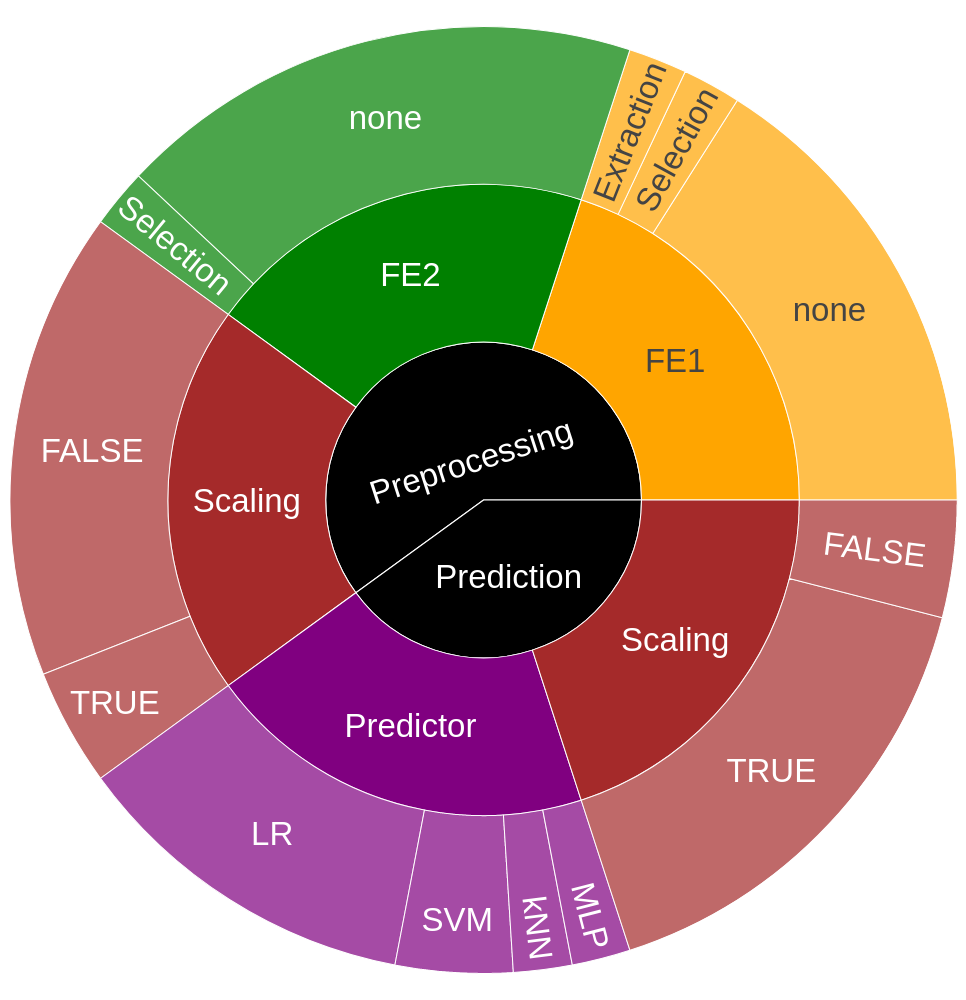
\includegraphics[width=\textwidth]{img/sunburst/cifar10.png}
    \caption{CIFAR-10}
  	\end{subfigure}
  	\begin{subfigure}[t]{0.3\textwidth}
    \centering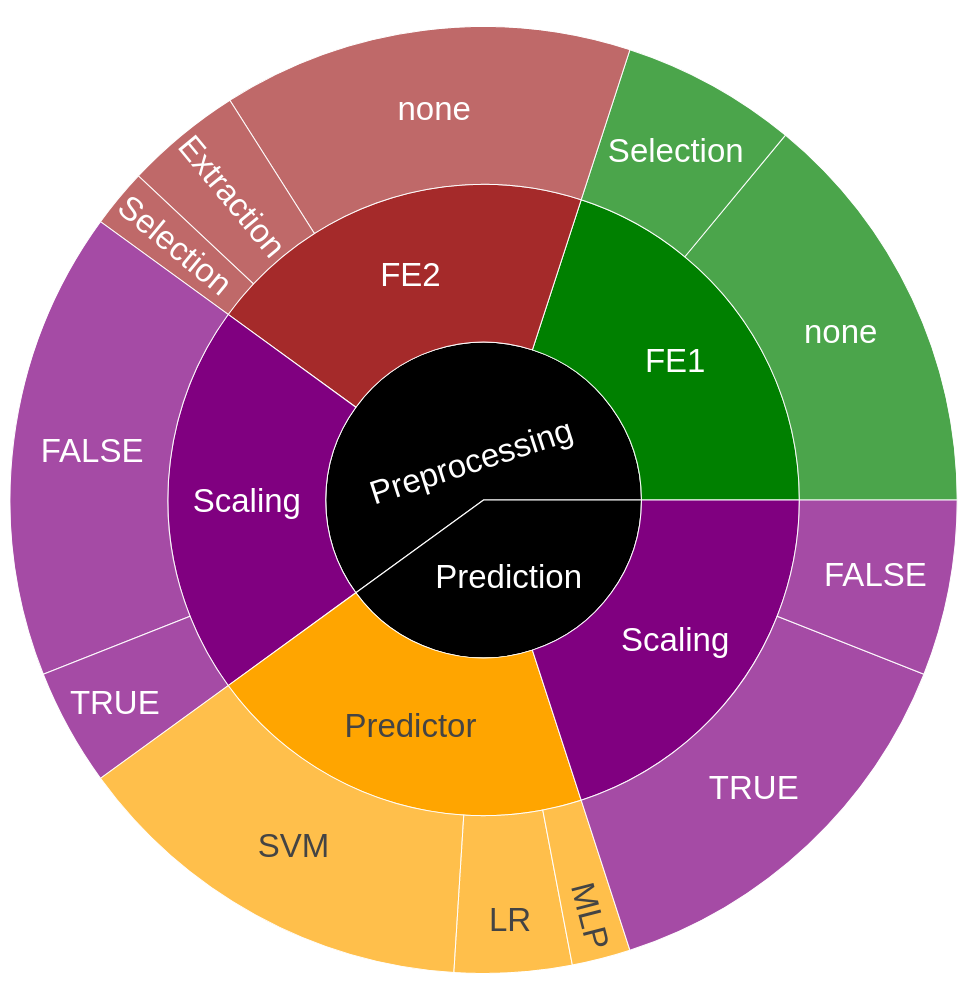
\includegraphics[width=\textwidth]{img/sunburst/fmnist.png}
    \caption{FMNIST}
  	\end{subfigure}
	\begin{subfigure}[t]{0.3\textwidth}
    \centering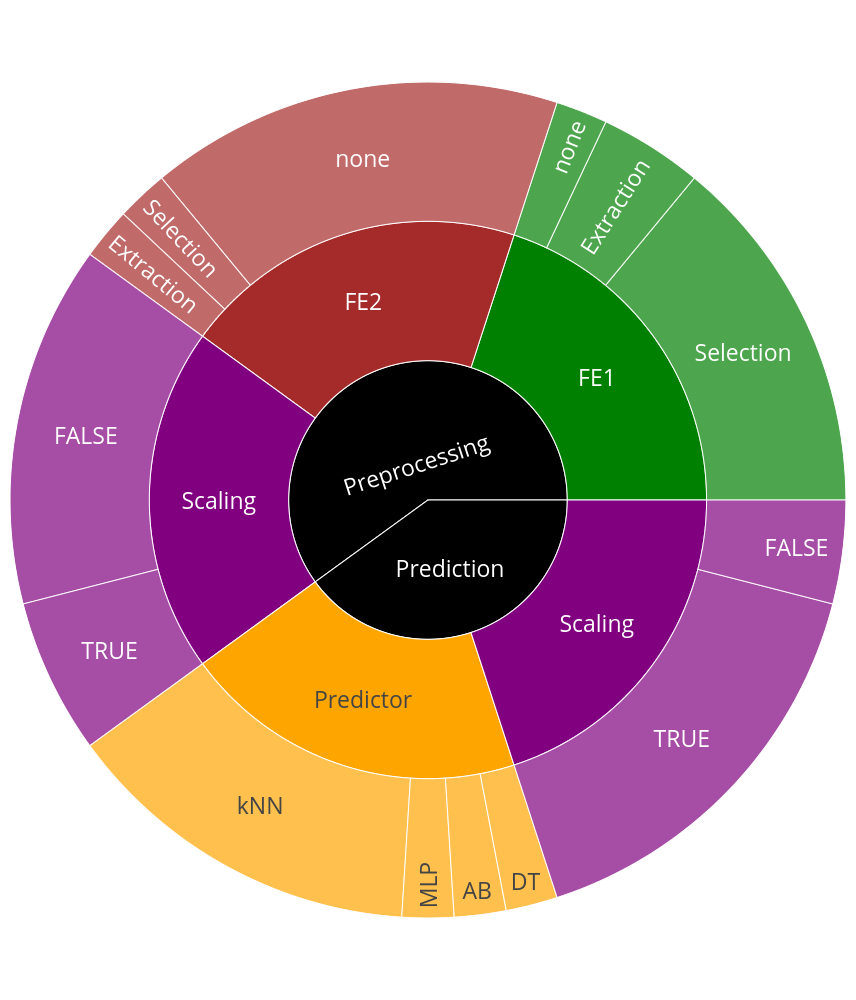
\includegraphics[width=\textwidth]{img/sunburst/svhn.png}
    \caption{SVHN}
  	\end{subfigure}

  	\begin{subfigure}[t]{0.3\textwidth}
    \centering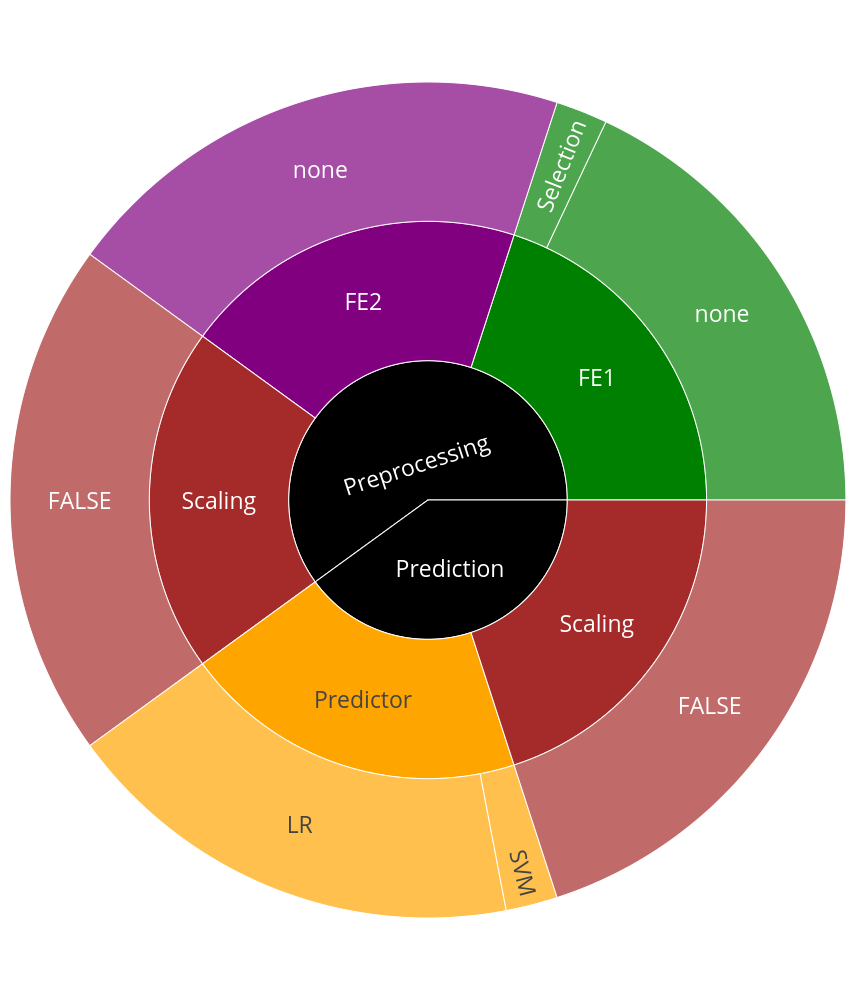
\includegraphics[width=\textwidth]{img/sunburst/lmrd.png}
    \caption{LMRD}
  	\end{subfigure}
  	\begin{subfigure}[t]{0.3\textwidth}
    \centering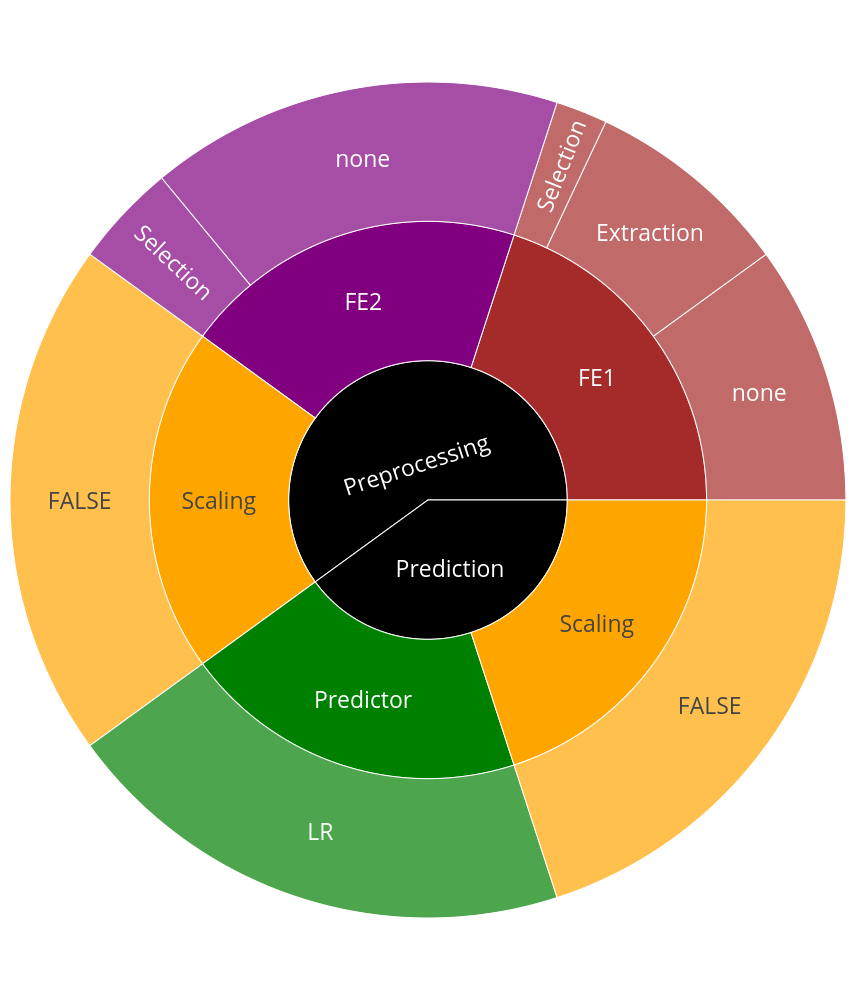
\includegraphics[width=\textwidth]{img/sunburst/reuters.png}
    \caption{Reuters}
  	\end{subfigure}
	\begin{subfigure}[t]{0.3\textwidth}
    \centering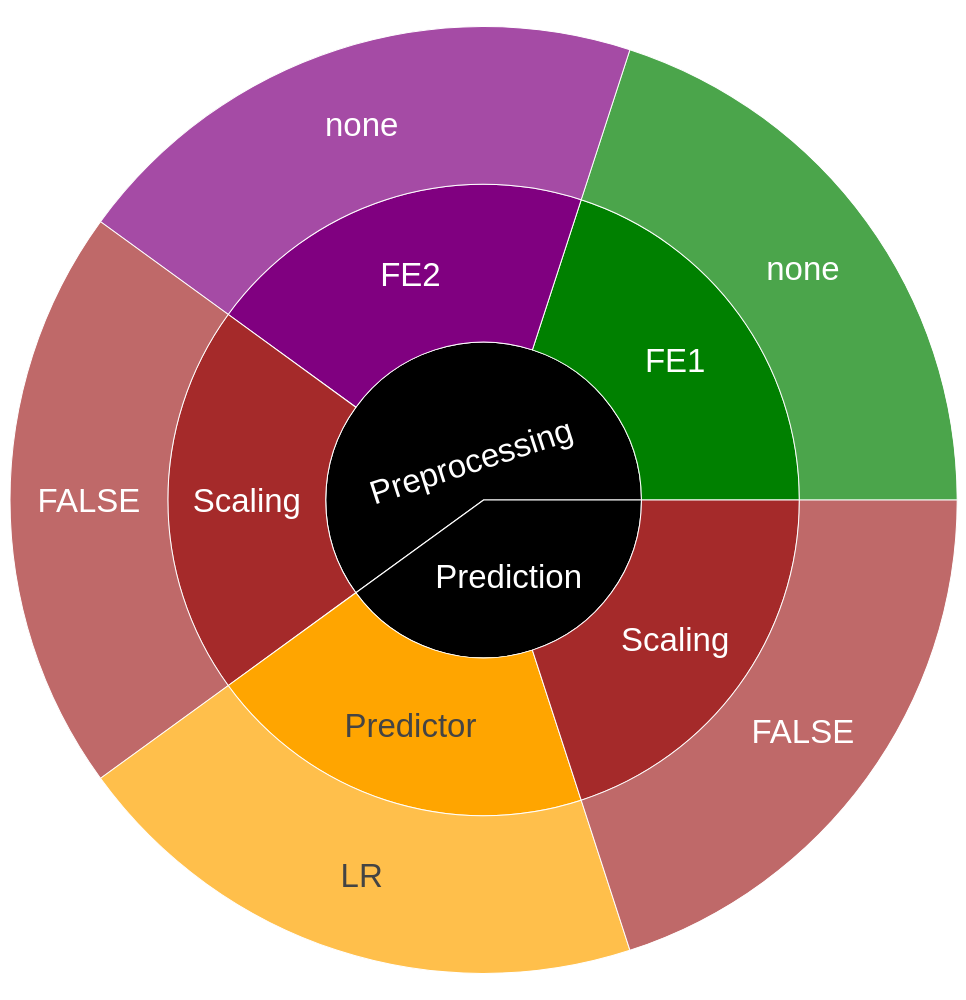
\includegraphics[width=\textwidth]{img/sunburst/agnews.png}
    \caption{AGNews}
  	\end{subfigure}

  	\begin{subfigure}[t]{0.3\textwidth}
    \centering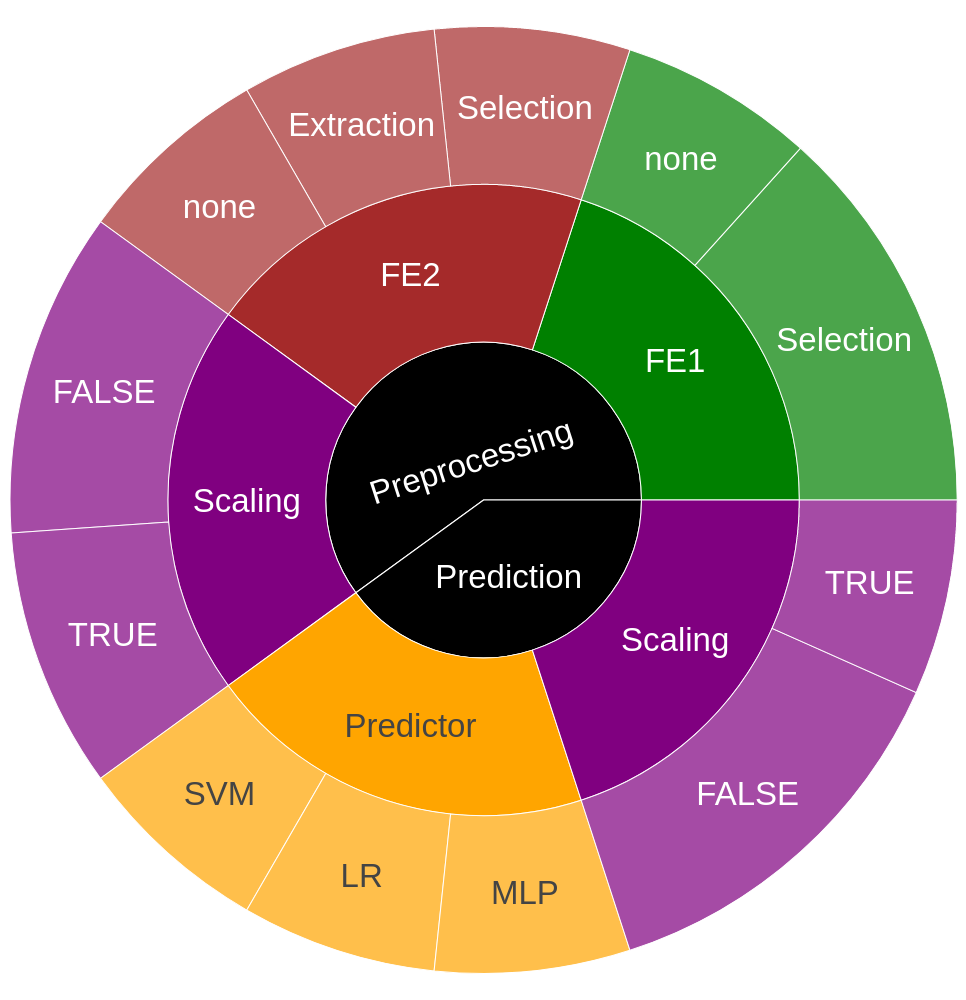
\includegraphics[width=\textwidth]{img/sunburst/natal.png}
    \caption{Natal}
  	\end{subfigure}
	\begin{subfigure}[t]{0.3\textwidth}
    \centering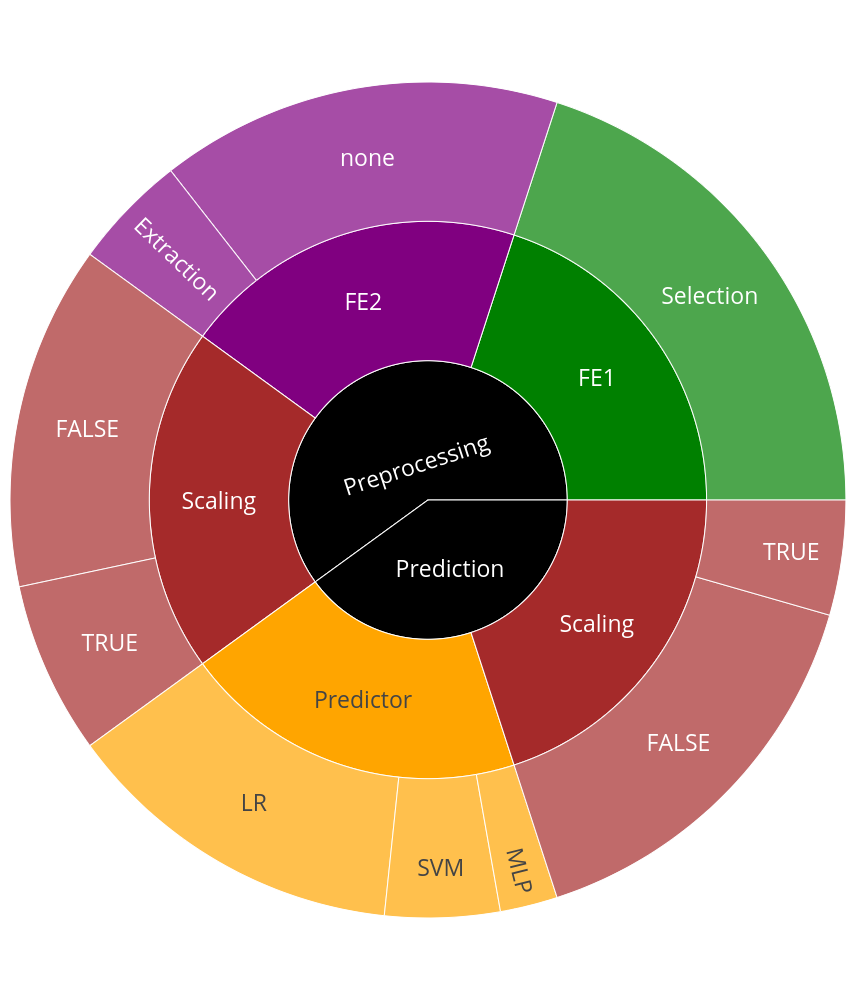
\includegraphics[width=\textwidth]{img/sunburst/boston.png}
    \caption{Boston}
  	\end{subfigure}

    \caption{Pipeline composition for each dataset.}
    \label{fig:dataset_composition}
\end{figure*} % Appendix E, F

\end{document}
